\documentclass[a4paper]{report}

% Bibliography management
\usepackage{natbib}
\bibpunct{[}{]}{,}{a}{}{;}

% IAM templates
\usepackage{fancyheadings}
\usepackage{iamdip}

% Figures
%\usepackage{subfig}
\usepackage{caption, subcaption}

% Math packages
\usepackage{amsmath}
\usepackage{amsthm}
\usepackage{amssymb}
\usepackage{amsfonts}

% Bold math symbols
\usepackage{bm}

% Hyperlinks
\usepackage{url}
\usepackage{hyperref}

% Code snippets
\usepackage{listings}

% PDF 
\usepackage[pdftex]{graphicx}
\usepackage{pdfpages}

% Quotations
\usepackage{dirtytalk}

% Colored text
\usepackage{xcolor}
\usepackage{soul}


% Page setup
\headrulewidth 0.5pt \addtolength{\headheight}{5pt}
\lhead[\fancyplain{}{\rm\thepage}]{\fancyplain{}{\rightmark}}
\rhead[\fancyplain{}{\leftmark}]{\fancyplain{}{\rm\thepage}}
\cfoot{}

% Custom commands
\newcommand \todo[1]{{\large \textbf{\textcolor{red}{#1}}}}
\newcommand \const[1]{\mathrm{#1}}
%\newcommand \vectr[1]{\mathbf{#1}}
%\newcommand \matr[1]{\mathbf{#1}}
\newcommand \vectr[1]{\bm{#1}}
\newcommand \matr[1]{\bm{#1}}
\newcommand{\R}{\mathbb{R}}
\DeclareMathOperator*{\argmax}{argmax}
\DeclareMathOperator*{\argmin}{argmin}

% Path setup
\graphicspath{{../Figures/}}

\begin{document}

	\pagestyle{fancyplain} \thispagestyle{empty}
	
	\title{Learning Structure from Motion \\ \textcolor{red}{DRAFT}}
	\author{Adrian W\"alchli}
	\betreuer{Prof. Dr. Paolo Favaro}
	\ort{Bern}
	\datum{2017}
	
	\pagenumbering{roman} \setcounter{page}{1}
	\maketitle
	
	% Abstract
	\newpage
	\thispagestyle{empty}
\vspace{8cm}
\noindent
{\centerline {\bf \large Abstract}}
\vspace{1cm}
\noindent

Abstract
	\newpage{\pagestyle{empty} \cleardoublepage}
	
	% Acknowledgements
	\thispagestyle{empty}
\vspace{8cm}
\noindent
{\centerline {\bf \large Acknowledgements}}
\vspace{1cm}

\noindent
I would like to express my deeply felt gratitude to the people who have supported me throughout my master studies and this thesis.
In particular, I would like to thank 

\begin{itemize}
	\item my supervisor Prof.\@ Paolo Favaro for his continuous support and guidance,
	
	\item the PhD students of the Computer Vision Group, that is, Simon, Givi, Meiguang, Xiaochen, Qiyang, Mehdi and Attila, 
	
	\item my brothers, parents and grandparents, 
	
	\item and a bunch of other great friends and colleagues that, in some form or another, contributed to my wellbeing during my master studies: Armin, Susanne, Florian, Raoul, Amanda, Ren\'e, Lars, Peter, Siavash.
	
\end{itemize}

	\newpage{\pagestyle{empty} \cleardoublepage}
	
	% Begin page numbering
	\pagenumbering{roman} \setcounter{page}{1}
	
	% Table of contents
	\tableofcontents
	\newpage{\pagestyle{empty} \cleardoublepage}
	
	% Main document
	\pagenumbering{arabic} \setcounter{page}{1}
	\pagestyle{fancy}
	
	\chapter{Prior Work}

	\todo{Add text that introduces the chapter}
	
		
	\section{04/2017 - SfM-Net}

		\cite{SFMNET} implement a deep learning approach to structure from motion. 
		Their architecture consists of two subnetworks:
		\begin{itemize}
			\item \textbf{Structure }
				\\
				Learns per-frame depth.
				The input is a single frame. 
				The output of the CNN is a cloud of 3D points, one for each pixel value in the input image.
			\item \textbf{Motion}
				\\
				The input is a pair of frames.
				The CNN computes a set of $K$ segmentation masks for moving objects. 
				Using these masks, each pixel is assigned to an object specific transformation given by a rotation and a translation.
				In addition, camera rotation and translation are computed using the features of the inner layers.
		\end{itemize}
		Given a pair of images, the forward operation of the network works as follows:
		\begin{enumerate}
			\item The structure network computes the point cloud for the first frame.
			\item The motion network computes the object transformations as well as the camera transformation using both frames.
			\item The point cloud is transformed using the learned object transformations and masks.
			\item The transformed 3D points are re-projected to 2D using the learned camera transformation between the two frames.
		\end{enumerate}
		The transformed point cloud corresponds to the depth of the second frame.
		Optical flow can be computed directly from the re-projected points.
		
		The authors of the paper propose various modes of supervision to evaluate the architecture and to handle ambiguities in the reconstruction due to the ill-posed problem:
		\begin{itemize}
		\item \textbf{Self-supervision}
			\\
			No ground truth is given.
			The loss is defined by the brightness constancy constraint of the second frame warped to the first frame using the predicted optical flow.
			For this mode, they use the {KITTI} 2012/15 datasets
		\item \textbf{Depth}
			\\
			Ground truth is given in the form of depth for each pixel.
			This can be acquired for example by a Kinect sensor.
			They use the {RGB-D SLAM} dataset for ground truth depth.
			This helps to improve camera motion estimation. 
		\item \textbf{Camera motion}
			\\
			Camera motion is given as ground truth in form of a rotation and translation matrix.
			The relative transformation between predicted and ground truth transformation is 
		\item \textbf{Optical flow and object motion}
			\\
			They use this type of supervision with the MoSeg dataset which contains ground truth segmentation for each frame.
			This dataset contains more non-rigid body transformation.
			They evaluate the quality of the object motion mask by Intersection over union (IoU).
		\end{itemize}
		
	\section{07/2016 - Unsupervised CNN for Single View Depth Estimation}
	
		The work of \cite{garg2016} implements a autoencoder on stereo pair images to predict depth from a single image.
		Their architecture consist of the following parts.
		\begin{itemize}
			\item \textbf{Encoder}
				\\
				Takes a single image as input. 
				At training time, this is the left image of a stereo pair.
				The output is the predicted disparity map (scaled inverse depth).
			\item \textbf{Decoder}
				\\
				The decoder is only used at training time.
				It takes two inputs: The predicted disparities from the encoder and the right image of the stereo pair.
				The right image is warped using the displacements and compared to the encoder input (left image) using the color constancy error (photometric error).
		\end{itemize}
		Since the stereo pair is rectified, the disparity is a displacement along the scanline of the images.
		Thus the decoder implements a simple geometric transformation that does not need to be learned.
		At test time, only the encoder network with a single image as input is used.
		
		As noted by the author, there are standard stereo algorithms that produce disparity maps.
		However, these methods can not deal with distortions such as lens flare, motion blur, shadows, etc.
		The idea is that a neural network could learn to deal with such problems that occur in natural images.
		
		The dataset they use is {KITTI} which they augment by random crops, color channel scaling, and flipping the images.
		
		\section{05/2017 - A Survey on Structure from Motion}
		
			\cite{survey2017} give a very good and concise definition of structure from motion:
			
			\say{The structure from motion (SfM) problem in computer vision is the problem of recovering the three-dimensional (3D) structure of a stationary scene from a set of projective measurements, represented as a collection of two-dimensional (2D) images, via estimation of motion of the cameras corresponding to these images.}
			
			The three basic steps of SfM are:
			\begin{itemize}
				\item Feature detection, extraction and matching
				\item Camera motion estimation
				\item Recovery of 3D structure
			\end{itemize}
			
			\paragraph{Bundle adjustment} 
				This technique simply considers to minimize the re-projection error of the unknown 3D points and camera matrices.
				The re-projection error is formulated as the euclidean distance between the known image coordinates and the projection of the unknown points using the unknown camera matrices.
				As stated by \cite{survey2017}, the problem is non-convex and in practice, common optimization algorithms achieve only a poor local minimum.
				
			\paragraph{The eight point algorithm}
				The eight point algorithm, introduced by \cite{longuet1981}, is an algorithm that computes the \emph{fundamental matrix}.
				This matrix describes the relationship between corresponding points in the image planes of two cameras with different relative pose.
				The 
			
			\paragraph{Factorization methods}
				The first method proposed by \cite{tomasi1992factorization} only works with an orthographic camera model.
				A measurement matrix $W \in \mathbb{R}^{2n \times m}$ is defined as
				\begin{equation}
					W =
					\begin{bmatrix}
						x_{11} & \cdots & x_{1m} \\ 
						\vdots & \ddots & \vdots \\ 
						x_{n1} & \cdots & x_{nm} \\ 
						y_{11} & \cdots & y_{1m} \\ 
						\vdots & \ddots & \vdots \\ 
						y_{n1} & \cdots & y_{nm}
					\end{bmatrix}. 
				\end{equation}
				It contains the 2D coordinates of the $m$ orthographically projected 3D points for each of the $n$ cameras.
				Under the assumption that the origin of global coordinate system is located at the center of the point cloud, the matrix $W$ can be factorized into
				\begin{equation}
					W = RS,
				\end{equation}
				where $R \in \mathbb{R}^{2n \times 3}$ contains the orientation vectors of each camera and $S \in \mathbb{R}^{3 \times m}$  are the 3D points.
				As described by \cite{tomasi1992factorization}, this factorization can be achieved using the singular value decomposition (SVD) as $W = U \varSigma V^\top$ and deriving $R$ and $S$ from $U$, $V$ and $\varSigma$.
				\todo{Add more details? Less details?}
				This factorization method was later extended by \cite{sturm1996factorization} for perspective cameras.
				
			\paragraph{Camera location estimation}
				To estimate the location and orientation of the cameras, one needs to find the rotation matrices $R_i \in \mathbb{R}^{3 \times 3}$ and translations $t_i \in \mathbb{R}^{3}$ for each of the cameras.
			
		\section{2015 - PoseNet}
		
			The PoseNet, as proposed by \cite{kendall2015posenet}, is a CNN that performs regression for the location and orientation of the camera given a single image as input.
			It outputs a 7D vector that describes the pose $p = [x, q]^\top$ as the camera location $x$ (3D) and orientation $q$ (4D quaternion).
			They simultaneously learn location and orientation with the euclidean loss
			\begin{equation}
				\mathcal{L}(I) = 
				\left\|
					\hat{x} - x 
				\right\|_2 
				+ \beta 
				\left\| 
					\hat{q} - \frac{q}{\left\| q \right\|} 
				\right\|_2,
			\end{equation}
			where $\beta$ is a parameter to balance the expected error of pose and orientation.
			The architecture is a modified \emph{GoogleNet} with 23 layers which was trained on a classification task.
			They replace the last layers to perform regression instead of classification.
			
			Because CNNs require a large amount of training data, the authors apply transfer learning by pretraining the network on a different task with large datasets such as \emph{ImageNet} and \emph{Places}.
			Pose regression is performed using the pre-trained network and their own dataset called \emph{Cambridge Landmarks} with five scenes of camera motion in large scale outdoor areas.
			For this limited dataset, ground truth pose is available.
			A challenge that comes with this dataset is the clutter in form of moving pedestrians and cars.
			Also, due to the long trajectories, weather and lighting conditions change a lot.
			
			In their experiments they find that the system is robust to large spatial distance between camera samples.
			Also, from the visualization of the features they observe that the network does not only produce high response outputs for high level features, but is also sensitive to large textureless regions where {SIFT}-based approaches typically fail.
			
			The paper demonstrates that transfer-learning can be used for pose estimation when a large labeled dataset for training is not available and that the pre-trained network can learn pose information despite being forced to produce pose-invariant outputs.
			\todo{connection to other work?}
		
		\section{02/2017 - Relative Camera Pose Estimation Using Convolutional Neural Networks}
			By \cite{melekhov2017poseCNN}
			\\
			\todo{add summary}
		
		
		
		
		
	\newpage{\pagestyle{empty} \cleardoublepage}
	
	\chapter{Introduction}

	\section{Relative Camera Pose}
		Equations to transform pose in world coordinates to relative pose with respect to the coordinate frame of the first camera.

	\section{Rotation Metrics}
	\cite{huynh2009metrics}
	
	\section{Two-Frame Structure from Motion}
	
	\section{Multiview Structure from Motion}
	
	\section{Camera Pose and Transformations}
		The camera pose, also known as the \emph{extrinsic parameters}, is a combination of position and orientation.
		Together, they define a coordinate transformation from the camera coordinate frame to the world coordinate frame.
		Such a transformation is commonly represented by a translation vector $\vectr{t} \in \R^3$ and a rotation matrix $\matr{R} \in SO(3)$. 
		Together, they describe a rigid transformation which can also be written as a $4 \times 4$ matrix of the form
		\begin{equation}
			\matr{T} = 
			\begin{bmatrix}
				\matr{R} 	& \vectr{t} \\
				0 			& 1
			\end{bmatrix} 
			\in SE(3).
		\end{equation}
		\todo{Insert a figure showing: world coordinate frame, camera coordinate frame, transformation matrix}
		
		In Structure from Motion, there is not only one camera, but many cameras with different transformations.
		This is also the case in this work, but the sequence of transformations is ordered according to the path of the camera motion. 
		Specifically, we deal with a sequence of rotations $\matr{R}_1, \dots, \matr{R}_n$ and translations $\vectr{t}_1, \dots, \vectr{t}_n$. 
		Depending on how the poses are obtained, they are all relative to a common (world) coordinate frame.
		Sometimes it is useful to have the coordinate frame of the first camera transform be the common frame for all transformations.
		This can be achieved by applying the transformations
		\begin{align}\label{eq:relative_rotation_conversion}
			\begin{split}
				\matr{R}_{i}^\prime 	&= \matr{R}_{1}^{\top} \matr{R}_{i} \\
				\vectr{t}_{i}^\prime 	&= \matr{R}_{1}^{\top} (\vectr{t}_i - \vectr{t}_1)
			\end{split}
		\end{align}
%		\begin{equation}
%			\matr{R}_{i \rightarrow 1} 	= \matr{R}_{\text{w} \rightarrow 1} \matr{R}_{i \rightarrow \text{w}}
%										= \matr{R}_{1 \rightarrow \text{w}}^{-1} \matr{R}_{i \rightarrow \text{w}}
%										= \matr{R}_{1 \rightarrow \text{w}}^{\top} \matr{R}_{i \rightarrow \text{w}}
%		\end{equation}
%		\begin{equation}
%		\vectr{t}_{i \rightarrow 1} = \matr{R}_{1 \rightarrow \text{w}}^{\top} (\vectr{t}_i - \vectr{t}_1)
%		\end{equation}
		to get the new relative rotation $\matr{R}_{i}^\prime$ and relative translation $\vectr{t}_{i}^\prime$.
		Note that for $i = 1$ we obtain $\matr{R}_{1}^\prime = \matr{I}$ and $\vectr{t}_{1}^\prime = \vectr{0}$.
		
		\noindent\rule{2cm}{0.4pt}
		\todo{make good transition}
		
		So far, we have seen rotations represented as matrices. 
		However, it is redundant to describe rotations with nine numbers when in fact there are only three degrees of freedom for a three-dimensional rotation, i.e. two degrees for the orientation of the axis and one for the angle of rotation around the axis.
		It is also not straightforward to interpolate rotations in $SO(3)$, or to find the best approximation for a matrix that lies outside of $SO(3)$.\todo{citation needed}
		
		Below we discuss and compare three other popular representations used to describe rotations.
		A brief overview is also shown in table~\ref{tbl:comparison_representations_of_rotations}.
		\begin{table}
			\small
			\begin{center}
				\begin{tabular}{|l|p{2.5cm}|p{2.5cm}|p{2.5cm}|p{2.5cm}|}
					\hline
					& Euler angles & Matrix & Axis-angle & Unit quaternion \\ \hline
					Typical use case & Robotics, Avionics & Computer Graphics, Physics & Intermediate representation & Computer Graphics, Physics \\ \hline
					Constraint & None & Orthonormality & Unit norm axis & 4D unit sphere \\ \hline
					Disadvantage & Gimbal lock & Numerically unstable & & Less intuitive \\ \hline
					Interpolation & hard & hard & hard & easy \\ \hline
					Identity rotation & ambiguous & unique & ambiguous &unique \\ 
					\hline
				\end{tabular}
			\end{center}
			\caption[A comparison of representations for rotations]
					{A comparison of representations for rotations.}
			\label{tbl:comparison_representations_of_rotations}
		\end{table}
		
		\paragraph{Euler Angles}
%		The fact that rotations in 3D have three degrees of freedom means there are only three coordinates needed to identify a rotation. 
%		Euler angles are one such choice of coordinates.
		The Euler angles represent a rotation with three numbers 
		$\alpha, \beta, \gamma \in \left[0, 2\pi\right)$.
		There are many different conventions and definitions of these three angles and how they are applied.
		In this thesis, we apply the rotations in the following order. 
		The initial coordinate frame shall be denoted by $(x, y, z)$.
		\begin{enumerate}
			\item The coordinate frame is rotated around the $x$-axis with angle $\alpha$. 
			This results in a new coordinate frame $(x^\prime, y^\prime, z^\prime)$.
			\item Next, the system is rotated around the $y^\prime$-axis by angle $\beta$. 
			The new coordinate frame is $(x^{\prime\prime}, y^{\prime\prime}, z^{\prime\prime})$.
			\item Finally, we perform a rotation around axis $z^{\prime\prime}$ by angle $\gamma$ to obtain the desired orientation.
		\end{enumerate}
		Altogether these steps can be formalized by a multiplication of three matrices that define the rotations around the different axes. 
		The result is a rotation matrix
		\begin{equation}
			\matr{R}(\alpha, \beta, \gamma) =
			\matr{R}_{z^{\prime\prime}}^\gamma
			\matr{R}_{y^\prime}^\beta
			\matr{R}_{x}^\alpha
		\end{equation}
		defined by the Euler angles. 
		It can be shown that this representation covers all 3D rotations. \todo{citation needed}
		However, the Euler angle representation also comes with drawbacks.
%		For example, a linear interpolation in the Euler domain between two points $(\alpha_1, \beta_1, \gamma_1)$ and $(\alpha_2, \beta_2, \gamma_2)$ by varying a parameter $\lambda \in [0, 1]$ gives 
%		\begin{equation}
%			(\alpha, \beta, \gamma) = (1 - \lambda) (\alpha_1, \beta_1, \gamma_1) + \lambda (\alpha_2, \beta_2, \gamma_2).
%		\end{equation}
%		The rotations associated with the angles $(\alpha, \beta, \gamma)$ is not an optimal choice for an 
		
		
		\paragraph{Axis-Angle}\todo{TODO}
		
		\paragraph{Quaternions}
		Quaternions are four-dimensional numbers.
		They are an extension of the complex numbers\footnote{A more appropriate name is \emph{compound numbers}.\todo{disputable}}.
		Formally, a quaternion is defined as $\vectr{q} = w + \vectr{i}x + \vectr{j}y + \vectr{k}z$ where $w, x, y, z \in \R$ and $\vectr{i},\vectr{j}$ and $\vectr{k}$ are the basis elements of the quaternion space.
		The quaternion can also be written as a tuple $\vectr{q} = (w, x, y, z) \in \R^4$ by using the notation
		\begin{equation}
			\vectr{1} = 
			\begin{bmatrix}
				1 \\ 
				0 \\ 
				0 \\ 
				0
			\end{bmatrix},\quad
			\vectr{i} = 
			\begin{bmatrix}
				0 \\ 
				1 \\ 
				0 \\ 
				0
			\end{bmatrix},\quad
			\vectr{j} = 
			\begin{bmatrix}
				0 \\ 
				0 \\ 
				1 \\ 
				0
			\end{bmatrix},\quad
			\vectr{k} =
			\begin{bmatrix}
				0 \\ 
				0 \\ 
				0 \\ 
				1
			\end{bmatrix}.
		\end{equation}
		But quaternions are not just tuples of numbers. 
		They are equipped with a separate addition and multiplication.
		Addition is simply carried out element-wise as for vectors, whereas multiplication makes use of the distributive rule and the property
		\begin{equation}
			\vectr{i}^2 = \vectr{j}^2 = \vectr{k}^2 = \vectr{i}\vectr{j}\vectr{k} = -1.
		\end{equation}
		Furthermore, the norm of a quaternion is defined as
		\begin{equation}
			\lVert \vectr{q} \rVert = \sqrt{w^2 + x^2 + y^2 + z^2}.
		\end{equation}
		
		In this thesis, we are particularly interested in the subset of quaternions called the \emph{unit quaternions}. These are all the quaternions with unit norm, i.e. $\lVert \vectr{q} \rVert = 1$. 
		The quaternions of this form describe 3D rotations and can be parameterized by
		\begin{equation}
			\vectr{q} = 
			\cos\left(\tfrac{\theta}{2}\right) + 
			\sin\left(\tfrac{\theta}{2}\right) \left(a_1 \vectr{i} + a_2 \vectr{j} + a_3 \vectr{k}\right),
		\end{equation}
		where $\theta \in \R$ is the angle of rotation around a unit-length axis $\vectr{a} = (a_1, a_2, a_3) \in \R^3$.
		\todo{explain that quaternions are not unique representation of rotations, and that negative axis-angle is represented by the same quaternion}
	
	\section{Deep Feedforward Neural Networks}
		\todo{This summary is based on the deep learning book}
		\todo{show a figure for a feed forward network}
		A \emph{feedforward neural network} is a function mapping an input $\vectr{x}$ to an output $\vectr{y} = f(\vectr{x})$.
		For example, $\vectr{y} \in \{\text{dog}, \text{cat} \}$ could be the output of the function deciding whether an image $\vectr{x}$ contains a dog or a cat. 
		The reason it is called a \emph{deep network} is because $f$ is often a long chain of function compositions, e.g. 
		$f = f^{(n)} \circ  \ldots  \circ f^{(2)} \circ f^{(1)}$.
		The functions $f^{(1)}, \dots, f^{(n)}$ are called \emph{layers} and $n$ is the \emph{depth} of the network.
		Each layer performs a computation on the output of the previous layer, hence the name \emph{feedforward}.
		
		A feed forward network is best visualized as a graph\footnote{More precisely it is a DAG (directed acyclic graph). It does not allow loops.}, the so-called \emph{computational graph}.
		A node in the graph represents a single layer and the edges represent the flow of data (input/output).
		\todo{Should explain comp. graph in terms of neurons?}
		These networks build the foundation of deep learning.
		Why?
		Because in general $f$ is unknown and must be learned to solve a specific task.
		The practical approach to finding a suitable $f$ is to consider a family of functions $f_{\vectr{w}}$ defined by the \emph{parameters} $\vectr{w}$, also called \emph{weights}.
		For example, the layer $i$ in the network might be a linear function $f_{}^{(i)}(\vectr{x}) = \matr{W} \vectr{x}$ where the parameters of this layer are the elements of the matrix $\matr{W}$.
		
		The collective of all functions in the family is called the \emph{model}.
		To solve the task (e.g. classifying dogs and cats), one has to \emph{train} the model.
		In other words, one has to search through the space of all parameters $\vectr{w}$ to find the ones that perform the best.
		The performance is measured with the \emph{loss function} 
		$L(f_{\vectr{w}}(\vectr{x}), \vectr{y}) \in \R$ that compares the prediction 
		$\vectr{\hat{y}} = f_{\vectr{w}}(\vectr{x})$ with the \emph{ground truth} $\vectr{y}$ and gives a score how close they are.
		The ground truth comes from the dataset, which is the most important resource of knowledge for training a model.
		The dataset contains many samples $\vectr{x}^{(1)}, \dots, \vectr{x}^{(N)}$ each with a ground truth label 
		$\vectr{y}^{(1)}, \dots, \vectr{y}^{(N)}$, e.g. each dog image in the dataset has a label 'dog' and each image with a cat has the label 'cat'.
		
		The loss function is not only used to evaluate the performance of the model, but to find optimal parameters for the model as part of the training.
		In general, the objective is to minimize the loss function on the data, that is
		\begin{equation}\label{eq:optimal_parameter_neural_network}
			\vectr{w}^\ast = \argmin_{\vectr{w}} 
			\sum_{i = 1}^{N} 
				L(f_{\vectr{w}}(\vectr{x}^{(i)}), \vectr{y}^{(i)}).
		\end{equation}
		The resulting function $f_{\vectr{w}^\ast}$ is a solution that best satisfies the loss function on all the data.
		How can $\vectr{w}^\ast$ be found?
		A common way to minimize the loss is to use gradient descent.
		It is one of the most general purpose optimization algorithms.
		Gradient descent can find a local minimum of a function $F$ by iteratively stepping in the opposite direction of the gradient, which can be described by the update rule
		\begin{equation}
			\vectr{w} \leftarrow 
			\vectr{w} - \lambda \frac{\partial F(\vectr{w})}{\partial \vectr{w}}.
		\end{equation}
		The parameters $\vectr{w}$ converge close to a local minimum when a suitable learning rate $\lambda$ is chosen. \todo{citation needed / is "converge" the right word to use here?}
		In the context of deep learning, $F$ is the loss function evaluated over the training data.
		More precisely, the update rule is
		\begin{equation}\label{eq:gradient_descent_update_rule}
			\vectr{w} \leftarrow 
			\vectr{w} - \lambda 
			\frac{\partial}{\partial \vectr{w}}
			\sum_{i = 1}^{N} 
				L(f_{\vectr{w}}(\vectr{x}^{(i)}), \vectr{y}^{(i)}).
		\end{equation}
		One parameter update with gradient descent requires the model to be evaluated for the entire dataset.
		This is a very expensive operation and in practice it is most often unfeasible.
		\emph{Stochastic} gradient descent is a modification that performs the update for each sample, which means that the sum in equation~\ref{eq:gradient_descent_update_rule} is dropped and the update rule is simply
		\begin{equation}\label{eq:stochastic_gradient_descent_update_rule}
			\vectr{w} \leftarrow 
			\vectr{w} - \lambda 
			\frac{\partial L(f_{\vectr{w}}(\vectr{x}^{(i)}), \vectr{y}^{(i)})}{\partial \vectr{w}}
			.
		\end{equation}
		The following steps describe a typical training procedure of a feedforward network.
		\begin{enumerate}
			\item Define model $f_{\vectr{w}}$
			\item Initialize parameters $\vectr{w}$
			\item Loop over training samples $\vectr{x}^{(i)}$ %for $i = 1, \dots, N$
			\begin{enumerate}
				\item Forward operation: $\vectr{\hat{y}} = f_{\vectr{w}}(\vectr{x}^{(i)})$
				\item Compute loss $L(\vectr{\hat{y}}, \vectr{y}^{(i)})$
				\item Backward operation: Backpropagate the gradient of the loss 
				\item Update parameters
			\end{enumerate}
		\end{enumerate}
		The algorithm above trains the model using each sample from the dataset once.
		A complete run over the dataset is called one \emph{epoch}.
		To improve the fit of the model to the data further, one can iterate for multiple epochs.
		
		After training it is a good practice to evaluate the model on new data, the test set.
		This way we can measure how well the model generalizes.
		It is important that the model performs well on new data because in practice we are often limited in how much data we can collect for training.
		
		A remark on the above summary for feedforward neural networks:
		Training with samples that have a ground truth label is called \emph{supervised learning}.
		It is also possible to learn from data where labels are not available.
		This is called \emph{unsupervised learning}.
		However, the focus of this thesis lies in the supervised approach.
		

		\todo{Gradient computation with backpropagation}\\
		\todo{explain the term "neural"}
	
	\section{Recurrent Neural Networks}\label{sec:recurrent_neural_networks}
		\newcommand{\imagecourtesycolah}{Image courtesy Christopher Olah \mbox{\href{http://colah.github.io/}{(colah.github.io)}}}
		\todo{Need references to early works on RNNs}
		So far, we have looked at the feedforward network, which is function that maps an input $\vectr{x}$ to an output $\vectr{y} = f(\vectr{x})$.
		It will always compute the same output for the same input, independently of the input-output pairs it has seen before.
		Now consider a sequence $\vectr{x}_1, \dots, \vectr{x}_T$ of inputs (e.g. a sentence).
		How can we learn to predict an attribute that depends on the whole sequence (e.g. the sentiment of the sentence)?
		One way is to concatenate the sequence to one vector and use the feed-forward network.
		However, this will limit the sequence length to a fixed size and potentially requires more training data.
		\todo{need reference for this statement}.
		How do we model predictions for a variable sequence length?
		And what if we want also the output to be a sequence? 
		What if the output sequence needs to have a different length than the input sequence, such as in machine translation? 
		\todo{citation needed}
		
		This is where the recurrent neural network (RNN) comes into play.
		It is a function that maps each vector $\vectr{x}_t \in \R^n$ from the sequence to a hidden state
		\begin{eqnarray}
			\vectr{h}_t = R(\vectr{x}_t, \vectr{h}_{t-1}), & &t = 1, \dots, T
		\end{eqnarray}
		with the hidden state $\vectr{h}_{t-1} \in \R^d$ carried over from the previous prediction as a second input, where $d$ is called the \emph{hidden size} of the RNN. 
		The hidden state represents the accumulated knowledge from all previous inputs.
		This way, the output at each time step $t$ depends on the inputs from $\vectr{x}_1$ to $\vectr{x}_{t - 1}$.
		\begin{figure}[tb]
			\centering
			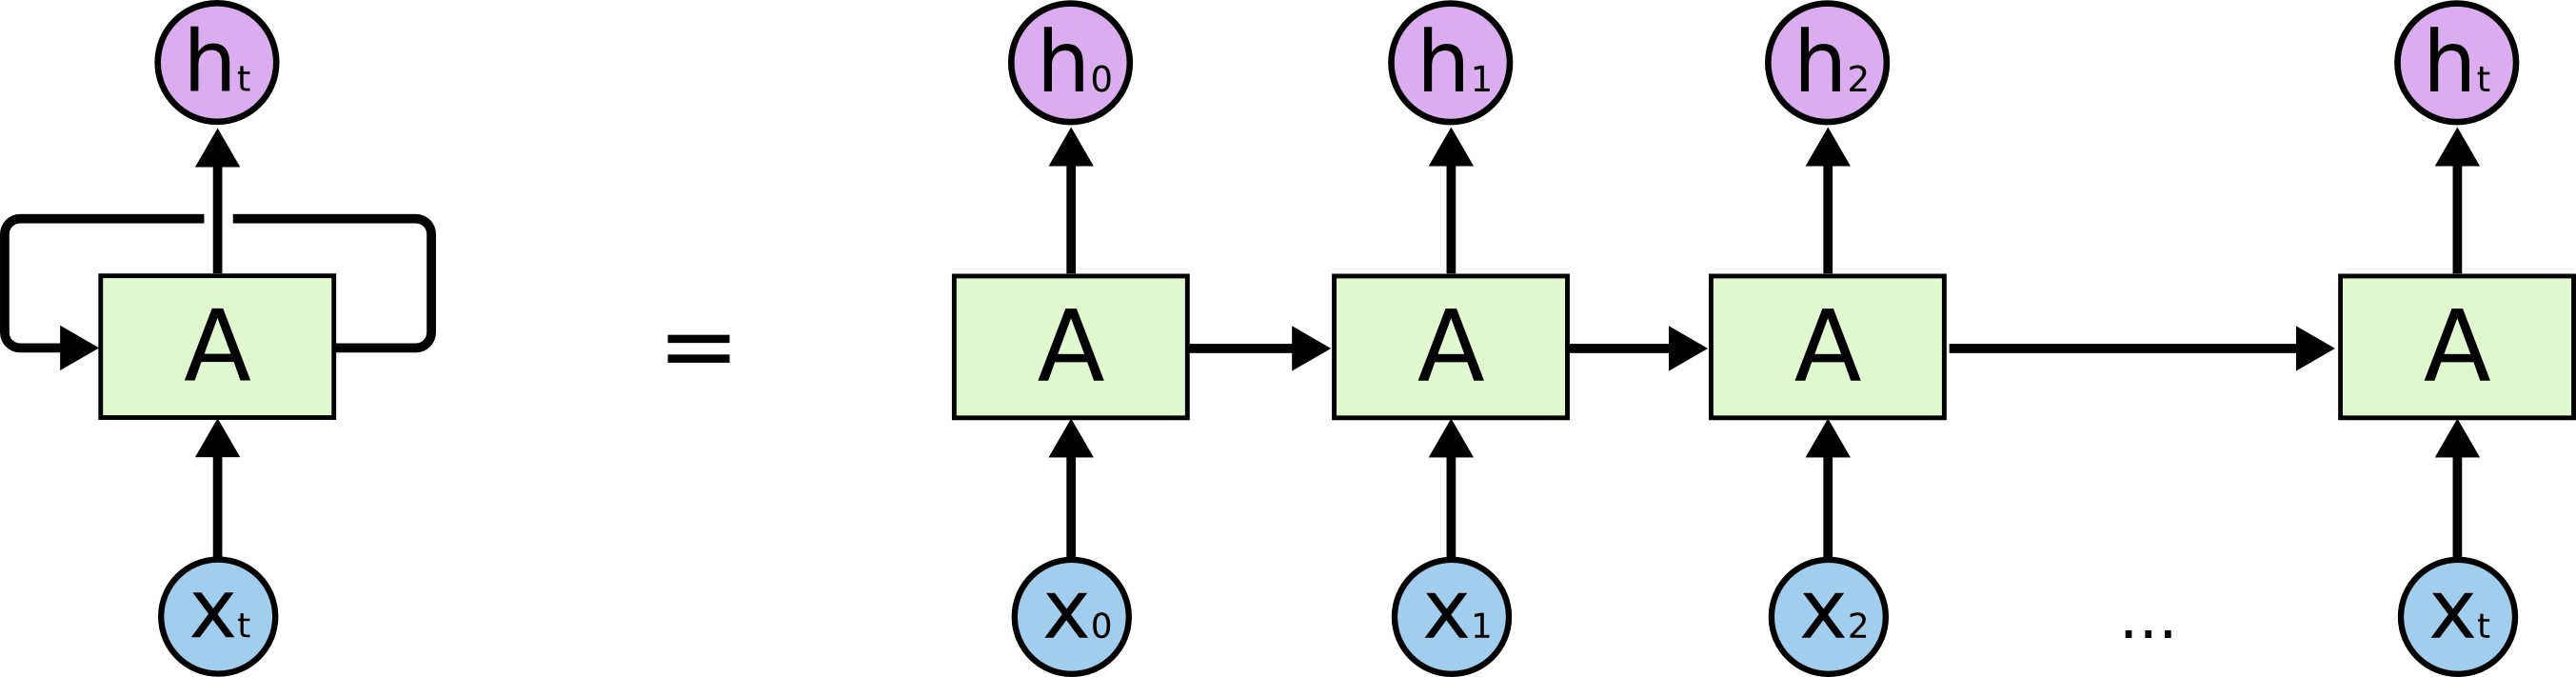
\includegraphics[width=0.9\linewidth]{Images/LSTM/RNN-unrolled}
			\caption[Unfolding the RNN]
			{Unfolding the RNN. Left: The RNN as a cyclic graph. 
				Right: Unfolded RNN for a number of timesteps.
				\imagecourtesycolah}
			\label{fig:RNN-unrolled}
		\end{figure}
		Figure~\ref{fig:RNN-unrolled} shows the RNN as a looping component.
		When unfolded, one can see the information flow from one state to the next.
		Note that it is possible to feed arbitrary sizes of sequences to the RNN.
		
		The simplest implementation of an RNN uses an affine transformation followed by a non-linear function:
		\begin{equation}
			\vectr{h}_t = 
			\tanh \left(
			\matr{W}
			\begin{bmatrix}
				\vectr{x}_t \\
				\vectr{h}_{t-1}
			\end{bmatrix}
			+ \vectr{b}
			\right)
		\end{equation}
		The weight matrix $\matr{W}$ has dimensions $d \times (n + d)$.
		Sometimes it is desirable to have an output that has a different size than the hidden state (e.g. for classification).
		In this case one can apply a second affine layer
		\begin{equation}
			\vectr{y}_t = \matr{V} \vectr{h}_t + \vectr{c}
		\end{equation}
		to obtain the prediction $\vectr{y}_t$.
		Otherwise we define the output as $\vectr{y}_t = \vectr{h}_t$.
		
		Training an RNN is not much different from a feed-forward network.
		The weights $\vectr{W}, \vectr{V}, \vectr{b}$ and $\vectr{c}$ are updated in the same fashion as for feed-forward networks using gradient descent on the loss function.
		Say we define a criterion $L_t(\vectr{y}_t, \vectr{\hat{y}}_t)$ for the loss between prediction and ground-truth at each time step $t$.
		Then, the total loss for the sequence is simply 
		\begin{equation}\label{eq:loss_for_rnn}
			L(\{\vectr{y}_1, \dots \vectr{y}_T\}, \{\vectr{\hat{y}}_1, \dots \vectr{\hat{y}}_T\}) = \sum_{t=1}^{T} L_t(\vectr{y}_t, \vectr{\hat{y}}_t).
		\end{equation}
		This loss will be used to compute gradients for updating the model parameters similar to feed-forward networks.
		
	\section{Gradient Computation for RNNs}\label{sec:gradient_computation_RNN}
		The gradient computation is almost the same as for feed-forward networks and the back-propagation algorithm can be applied by unfolding the RNN as shown in figure~\ref{fig:RNN-unrolled}.
		However, there is a problem with the gradient computation in the above version of the RNN (\cite{pascanu2013difficulty}, \cite{bengio1994learning}).
		For long sequences, the gradient norm can become very small and this hurts the training.
		The RNN is not able to learn long-term dependencies when the gradient vanishes.
		To see this, let's write down the full equation for the gradient:
		\begin{equation}\label{eq:gradient_computation_RNN}
			\frac{\partial L}{\partial \vectr{w}}
			= \sum_{t=1}^{T} 
				\frac{\partial L_t}{\partial \vectr{w}}
			= \sum_{t=1}^{T} 
				\sum_{k=1}^{t} 
					\frac{\partial L_t}{\partial \vectr{y}_t}
					\frac{\partial \vectr{y}_t}{\partial \vectr{h}_t}
					\left(
						\prod_{j=k+1}^{t} \frac{\partial \vectr{h}_j}{\partial \vectr{h}_{j-1}}
					\right)
					\frac{\partial \vectr{h}_{k}}{\partial \vectr{w}}
		\end{equation}
		In the above equation, we have the product term that causes the problem when the sequence is very long.
		Note that the partial derivatives are Jacobian matrices when we take the derivatives of a vector-valued function with respect to a vector.
		Due to many multiplications, the gradient values drop exponentially.
		\todo{Need a better explanation why values are <1 and drop exponentially}
		A more complete analysis is provided in \cite{pascanu2013difficulty}.
		
	\section{The Long Short-Term Memory}
		\begin{figure}[tb]
			\centering
			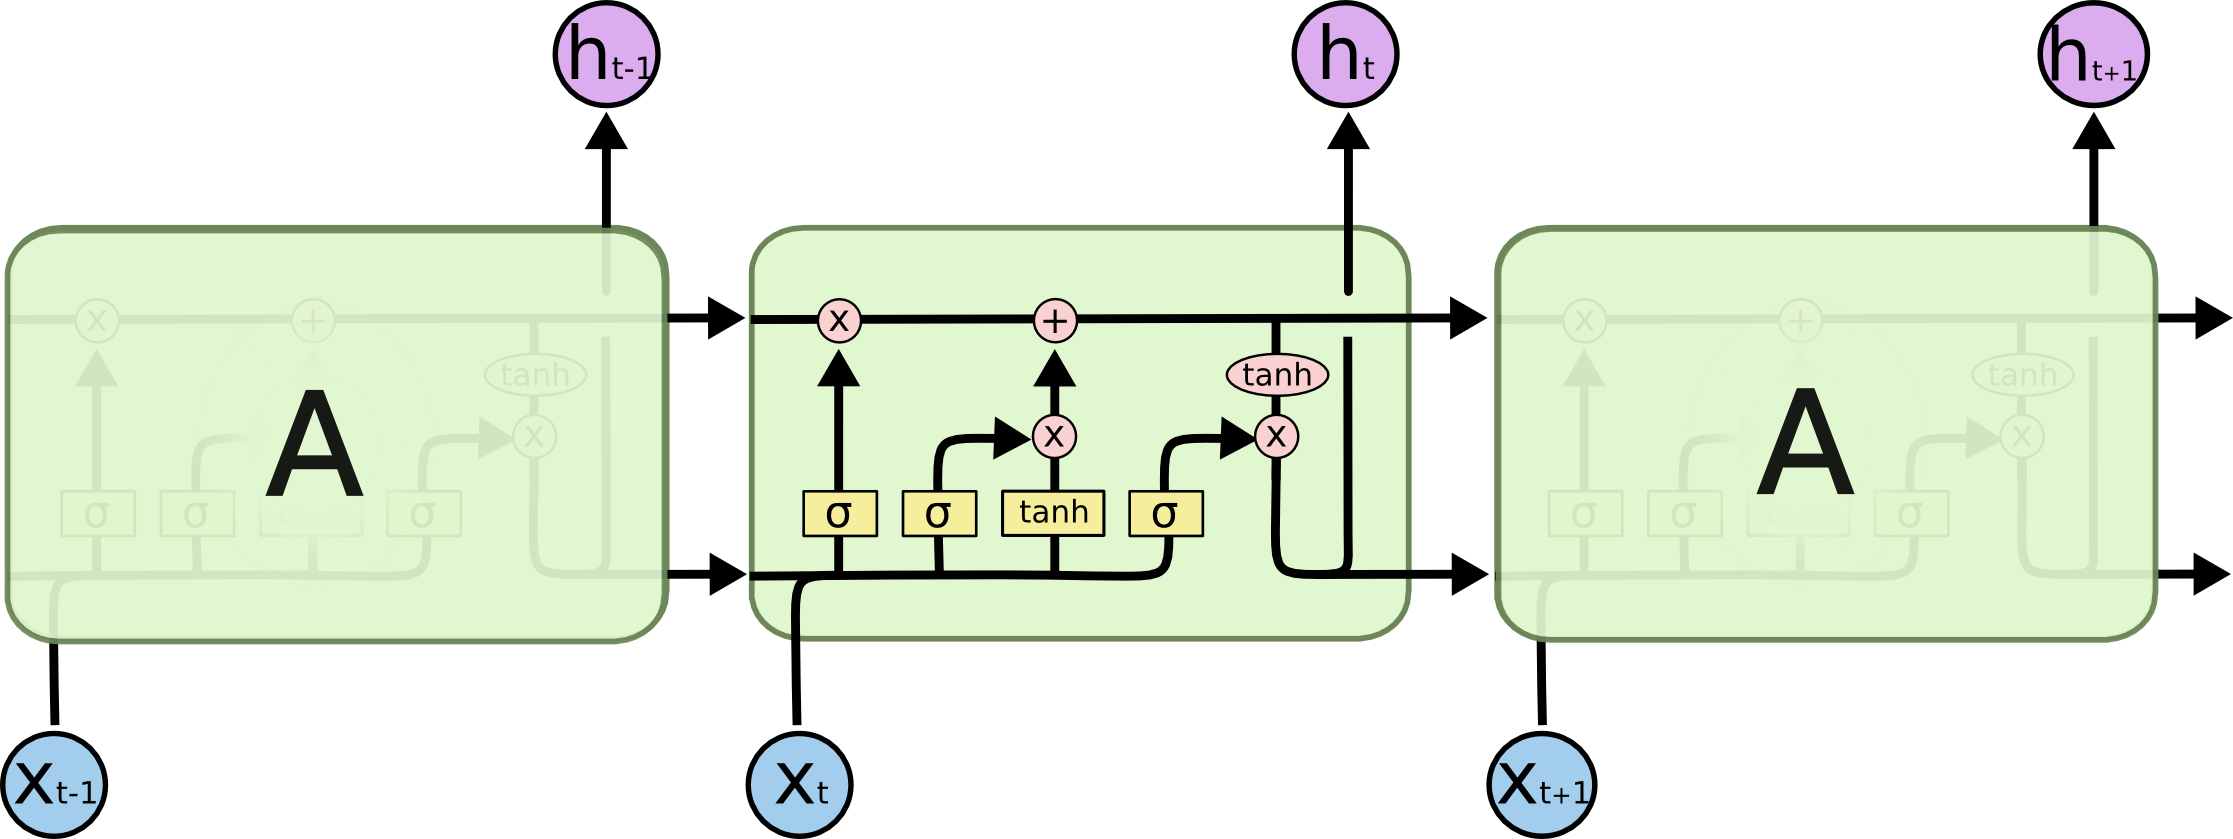
\includegraphics[width=0.9\linewidth]{Images/LSTM/LSTM3-chain}\\
			\vspace{5mm}
			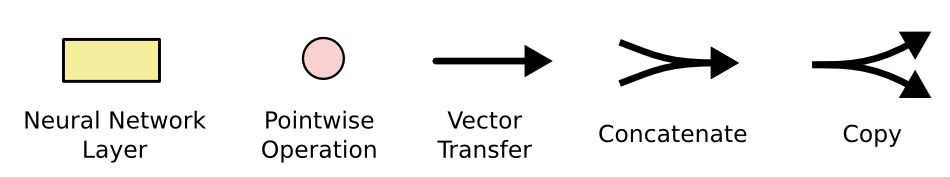
\includegraphics[width=0.5\linewidth]{Images/LSTM/LSTM2-notation}
			\caption[Unfolded LSTM cell]
					{Unfolded LSTM cell. 
					\imagecourtesycolah}
			\label{fig:LSTM3-chain}
		\end{figure}
		The Long Short-Term Memory (LSTM) is a version of the RNN that was designed to overcome the vanishing gradient problem described above, and it is also used in this thesis.
		As shown in figure~\ref{fig:LSTM3-chain}, it introduces four gates (in yellow) and an additional cell state variable that is carried over from one time step to the next.
		The recurrence can be formulated as a function 
		% $R \colon \R^n \times \R^d \times \R^d \rightarrow \R^d \times \R^d$
		\begin{align}\label{eq:LSTM_recurrence}
			(\vectr{h}_t, \vectr{c}_t) = R(\vectr{x}_t, \vectr{h}_{t-1}, \vectr{c}_{t-1}), & & t = 1, \dots, T.
		\end{align}
		More precisely, the hidden state and cell state are computed as follows:
		\begin{align}\label{eq:Vanilla-LSTM-Definition}
			\begin{split}
				\begin{bmatrix}
					\vectr{i} \\ 
					\vectr{f} \\ 
					\vectr{o} \\ 
					\vectr{g}
				\end{bmatrix}
				&=
				\begin{bmatrix}
					\sigma \\ 
					\sigma \\ 
					\sigma \\ 
					\tanh
				\end{bmatrix}
				\left(
				\matr{W}
				\begin{bmatrix}
					\vectr{x}_t \\
					\vectr{h}_{t-1}
				\end{bmatrix}
				+
				\begin{bmatrix}
					\vectr{b}_i \\ 
					\vectr{b}_f \\ 
					\vectr{b}_o \\ 
					\vectr{b}_g
				\end{bmatrix}
				\right)
				\\
				\vectr{c}_t &= \vectr{i} \odot \vectr{g} + \vectr{f} \odot \vectr{c}_{t-1} \\
				\vectr{h}_t &= \vectr{o} \odot \tanh(\vectr{c}_{t})
			\end{split}
		\end{align}
		The matrix $\matr{W} \in \R^{4d \times (n + d)}$ contains the weights for the input- and hidden state transformations before each gate.
		It can be broken down into four parts:
		\begin{align}
			\matr{W} &=
			\begin{bmatrix}
				\vectr{W}_i \\ 
				\vectr{W}_f \\ 
				\vectr{W}_o \\ 
				\vectr{W}_g
			\end{bmatrix}
		\end{align}
		We can see that there are three additional gates that control information flow with a sigmoid activation.
		If the sigmoid output is one, all information is let through, otherwise no information passes the gate. 
		
		The first is the input gate $\vectr{i}$.
		It controls how much information should be collected from the current input and hidden state.
		The second is the forget gate $\vectr{f}$, which will learn what information should be discarded from the previous cell state.
		Finally, the output gate $\vectr{o}$ regulates the amount of information that goes to the output $\vectr{h}_t$.
		
	\section{Training RNNs}
		% Intro: Two parts - optimization algorithm and how inputs/outputs are defined
		
		\paragraph{Optimization Procedure}
		In order to use the loss function to update the model weights, one has to specify an optimization algorithm.

		\todo{connect}
		
		There are several ways an RNN can be trained.
		First of all, one can distinguish the type of input-output relationship for RNNs.
		
		\paragraph{Input to Output Mapping}
		In section~\ref{sec:recurrent_neural_networks} it was assumed that for each time step $t$ there is an input $\vectr{x}_t$ and an output $\vectr{h}_t$.
		This is the most general setup for an RNN and we refer to it as \emph{many-to-many}. 
		
		For some tasks, it might not be suitable to have an input at each time, or an output at each time.
		On the other hand, the RNN is not a feedforward network in the time axis and thus does not allow a modification to remove inputs or outputs at certain time steps.
		However, this does not mean that one has to use all outputs for computing loss and gradients.
		For example, if we wish to predict the sentiment of a sentence, we can feed each word to the RNN and and ignore all outputs except the last one and use that for backpropagation of the gradient.
		We refer to this method as \emph{many-to-one}.
		If there is only one input available, but the output must a sequence (\emph{one-to-many}), one possibility is to simply feed the same input for all time steps.
		An example for this method is image captioning, where the input is an image and the output is a description of the image in form of a sentence. \todo{reference to a work on image captioning}
		Finally, the \emph{one-to-one} setting is a combination of the two above.
		
		\paragraph{Signaling Output} 
		Instead of ignoring certain outputs and only using the ones needed, an alternative is to use a special input symbol $\vectr{e}$ to explicitly signal that an output should be written.
		This special token has to be encoded with the same dimensionality as the other inputs. 
		Its numerical value can be fixed before training (as a hyperparameter) or it can be part of the model parameters and be learned.
		For example, in the sentiment analysis example from before, the token can be used as an end-of-sequence symbol to mark the end of a sentence.
		In general, the symbol does not necessarily have to be used at the end of a sequence.
		It can be inserted whenever an output is needed.
		An application of this is shown in an experiment later in the thesis. 
		\todo{Explicitly refer to the section}
		
		\paragraph{Truncated Backpropagation}
		As discussed in section~\ref{sec:gradient_computation_RNN}, gradient computation over long sequences can cause vanishing or exploding values that hinder the learning process during training.
		The LSTM was designed to addressed this issue, but backpropagation over very long sequences is still computationally expensive.
		As a compromise, one can choose to backpropagate only a certain amount of time steps.
		This is called \emph{truncated backpropagation through time} or TBPTT.
		In order to save memory and reduce computation, one can choose to limit the gradient computation through time.
		This is called \emph{truncated backpropagation through time (TBPTT)}. 
		Say the sequences have a length of $T$ and the number of time steps to backpropagate is $\tau \leq T$.
		To compute the gradient only back to $T - \tau$, we can replace the start indices for $t$ and $k$ in the sums of equation~\ref{eq:gradient_computation_RNN} with $T - \tau$.
		Obviously, this is an approximation of the full gradient over all time steps.
		The RNN is not forced to learn dependencies back in time longer than $\tau$ steps and thus we can not expect it to do so.
		\todo{mention where this is used later in thesis}
		
		A specific application of TBPTT is for training on one continuous data stream instead of many shorter sequences.
		For example, if the goal is to train an RNN to generate natural text, it needs to remember the context over multiple sentences.
		To do this, one can concatenate the data from all text documents to one very long sequence.
		During training, we can forward subsequences consecutively and backpropagate $\tau$ steps.
		After each backpropagation, the hidden state $\vectr{h}_t$ (or $(\vectr{h}_t, \vectr{c}_t)$ in the case of LSTM) is carried over to the next subsequence as initial state.
		This way, there is always information available from the past even though the gradients are never propagated to the very beginning of the sequence.
		\todo{mention where this is used later in thesis}
		
		\paragraph{Ground Truth}
		How ground truth is used depends heavily on the task at hand.
		In the aforementioned example for generating text, the RNN predicts the next word given the current word and the context (hidden state).
		Therefore, the ground truth data is the same as the input data except that it is shifted in time, e.g. $\vectr{y}_t = \vectr{x}_{t + 1}$.
		In this example, not only do the input and output have the same dimensionality (words are encoded as vectors), but the semantic meaning is also the same.
		This is of course not true for all applications of RNNs.
		In this thesis, the inputs are camera images (thousands of color values) and the outputs are poses (usually 6D or 7D vectors).
		The semantic gap is large since the pose is not directly encoded in the individual image, but in the motion between the frames.
		The pose is always relative to the first frame in the sequence.
		The RNN has to learn this directly from the ground truth, not from the input.
		
		
		% How the ground truth is used
		% 	Does ground truth have same dimensionality as input?, as hidden state?
		%
		
	\section{PyTorch}
		PyTorch is a deep learning framework for Python that comes with a rich tensor library.
		It differs from other libraries (TensorFlow, Caffe, Theano and more) in the sense that it builds the computational graph dynamically at runtime.
		This flexibility allows for controlling the computational flow while training or testing the network.
	\newpage{\pagestyle{empty} \cleardoublepage}
	
	\chapter{Experiments And Results}\label{chp:experiments-and-results}
	
%\section{Experiments and Results}
% Ablation studies
% Problem with "global" pose -> incremental pose
% Training
%	- Different learning rate for pretrained flownet
%	- Dropout Regularization
	This chapter presents all experiments conducted on the deep learning model that was introduced in chapter~\ref{chp:the_model}.
	The results shown here give useful insights that supplement the work of \cite{wang2017deepvo}.
	
	\section{Dataset Size and Dropout}
		We start by training the proposed model on the KITTI dataset on small subsequences of 25 frames. 
		Initially, the sequences are divided without overlap, that is, each video frame is part of exactly one subsequence.
		In addition, to simulate a dataset with more subsequences, the overlap is set to 20 frames (80\%). 
		This means that for each subsequence there is another one that differs by 5 frames.
		Table~\ref{tbl:kitti-overlap-and-dropout} compares the test error for models trained with and without overlap.
		\begin{table}[tb]
			\small
			\begin{center}
				\begin{tabular}{ccccrrr}
					\toprule
					\multicolumn{3}{c}{\textbf{Experiments}}	&	& \multicolumn{3}{c}{\textbf{Test error}} 		\\
					\cmidrule(lr){1-3} 					\cmidrule(lr){5-7}
					Length 			& Overlap 	& Dropout	&	& Total 	& Rotation	& Translation	\\ 
					\midrule
					25				& 0			& 0			& 	& 19.0293	& 0.4981	& 18.5312		\\ 
					25				& 20		& 0			&	& 16.5471	& 0.3913	& 16.1558		\\ 
					100				& 20		& 0			&	& 529.9459	& 39.8967	& 490.0493		\\ 
					100				& 80		& 0			& 	& 313.1278	& 47.8437	& 265.2841		\\ 
					100 			& 5			& 0.5		&	& 376.7666	& 43.1578	& 333.6088		\\ 
					%$20\rightarrow120$ 	& 5		& 0.5		&	& 303.7696	& 39.4114	& 264.3582		\\
					$20\rightarrow100$ 	& 5		& 0.5		&	& 289.8579 	& 42.0427 	& 247.8152 		\\
					\bottomrule
				\end{tabular}
			\end{center}
			\caption[Experiments on KITTI: Overlap and dropout]
					{Experiments on KITTI: Overlap and dropout. 
					 Shown is the test error on sequence 10 for different overlap and dropout during training.
					 The evaluation on the test set is performed on sequences of the same size as seen during training, and without overlap.
					 In the last row, the sequence length grows by one frame every epoch.
					 Each model was trained with default parameters for 100 epochs, except the last one which was trained for only 80 epochs.
					 \label{tbl:kitti-overlap-and-dropout}}
		\end{table}
		After the same number of epochs, the test error is about 13\% lower for the model trained on overlapping sequences with a decrease of 21\% for rotation and 12\% for translation.
		The same experiment is repeated by training on sequences of 100 frames with overlap 20 vs. overlap 80. 
		% Total error decreases by about 40\%.
		The translation error decreases by almost 46\%, however, the rotation loss increases.
		A similar observation can be made when using dropout on the LSTM output (before the fully-connected layer), as seen in the second last row of table~\ref{tbl:kitti-overlap-and-dropout}.
		
		For the last experiment in table~\ref{tbl:kitti-overlap-and-dropout}, the sequence length grows by an increment of one frame every epoch, starting from 20 frames and stopping at 100 frames after 80 epochs.
		As we can see, this method of training in combination with the dropout gives the best overall loss on the test set.
		A possible explanation for this could be the that the learning process is faster for short sequences because the LSTM requires a less complex memory mapping in order to remember the coordinate transforms from earlier time steps, including the first one.
		A gradual refinement of such a mapping may be less challenging for the optimization as opposed to learning it directly from long sequences.
		\todo{Need more explanation here.}
		
		Although the numbers in the table can be used to compare the different experiments, they are not very insightful by themselves.
		From the sum of squared differences alone, it is not possible to understand how the error behaves across the sequence.
		For better visualization, we can compute the error at regular distance intervals along the estimated path.
		Figure~\ref{fig:kitti-avg-rotation-translation-error-vs-path-distance} shows translation and rotation errors for path distance on subsequences of the KITTI sequence 10.
		\begin{figure}
			\centering
			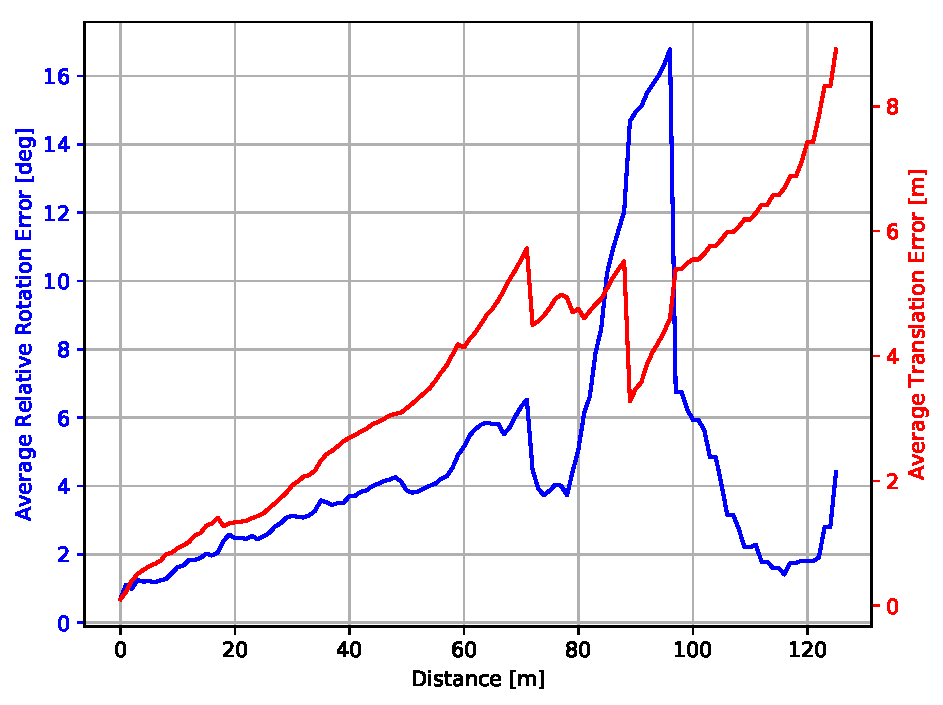
\includegraphics[width=0.7\linewidth]{Python-Plots/deepvo-KITTI/relative-rotation-and-translation-error-along-path-overlap80}
			\caption[Experiments on KITTI: Average rotation- and translation error vs. path distance]
					{Experiments on KITTI: Average rotation- and translation error vs. path distance.
					 The relative rotation- and translation error is evaluated at equal intervals along the subsequences of KITTI sequence 10.
					 The errors at the same distance are averaged over all sequences of that length.
					 \label{fig:kitti-avg-rotation-translation-error-vs-path-distance}}
		\end{figure}
		The relative rotation error is the angle of rotation around the axis corresponding to the relative rotation between estimated and ground truth pose.
		\todo{refer to equations introduced in previous chapter}
		
		\paragraph{Conclusion}
		From these experiments, we can conclude that sequence overlap and dropout have a positive impact on the generalization of translation estimates.
		Especially when training data is scarce, the overlap method can be utilized to artificially increase the dataset and reduce the error on the test data.
		
	\section{The Problem on Long Sequences}
		Ideally, we would like to train the model on sequences with an arbitrary number of frames.
		Due to the high cost of backpropagation in RNNs, the number of frames that can be processed at a time is limited by the available memory. 
		This allows to 
		\begin{table}[tb]
			\small
			\begin{center}
				\begin{tabular}{cccrrr}
					\toprule
					\multicolumn{2}{c}{\textbf{\#Frames}}	&	& \multicolumn{3}{c}{\textbf{Test error}} \\ 
					\cmidrule(lr){1-2} 									\cmidrule(lr){4-6}
					Training 		& Test 			&	& Total 	& Rotation	& Translation	\\ 
					\midrule
					25				& 25			&	& 16.5471	& 0.3913	& 16.1558		\\
					25				& 100			&	& 1060.7528	& 37.6196	& 1023.1332		\\
					100				& 100			&	& 529.9459	& 39.8967	& 490.0493		\\ 
					\bottomrule
				\end{tabular}
			\end{center}
			\caption[Experiments on KITTI: Testing on longer sequences]
					{Experiments on KITTI: Testing on longer sequences. 
					 When testing on sequences with more frames, the error becomes extremely high compared to the model trained on 100 frames.
				 \label{tbl:kitti-testing-on-longer-sequences}}
		\end{table}

		\begin{figure}
			\centering
			\begin{subfigure}[b]{0.5\linewidth}
				\centering
				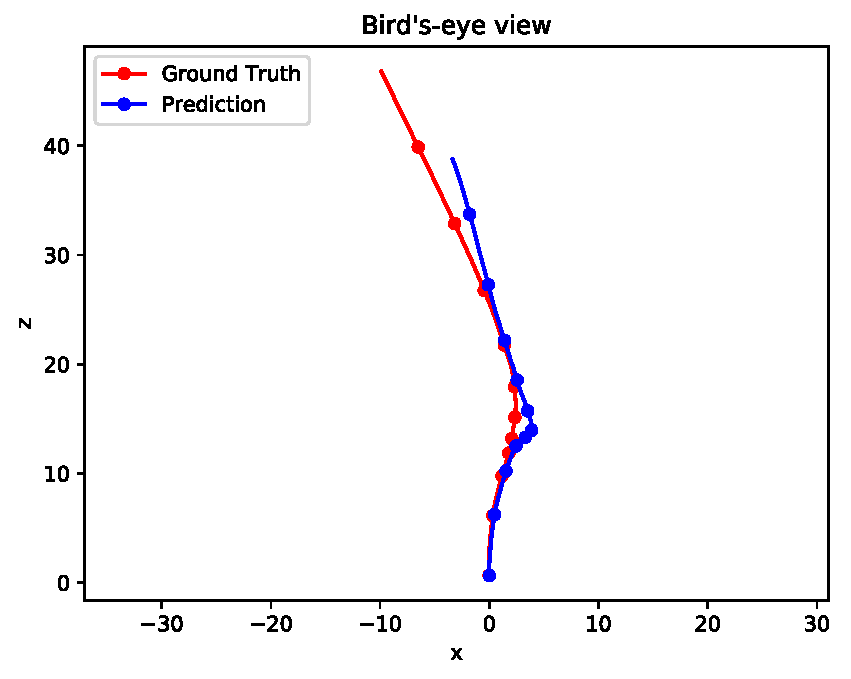
\includegraphics[width=\linewidth]{Experiments/trained-on-25-frames}
				\caption{
					\label{fig:0}
				}
			\end{subfigure}%
			\begin{subfigure}[b]{0.5\linewidth}
				\centering
				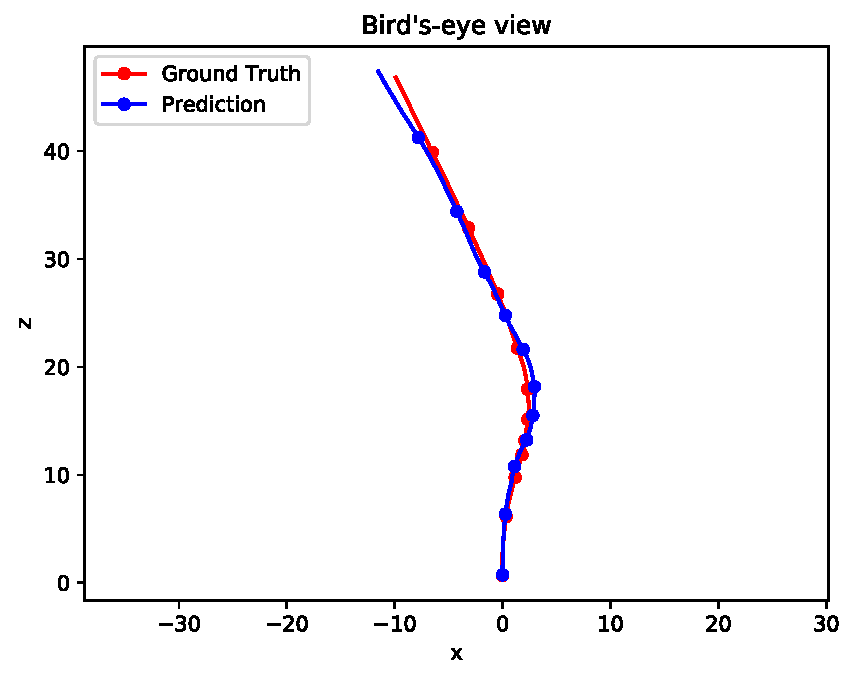
\includegraphics[width=\linewidth]{Experiments/trained-on-100-frames}
				\caption{
					\label{fig:1}
				}
			\end{subfigure}%
			\caption[Training and testing on different sequence length]
					{Training and testing on different sequence length. 
				 Two models tested on a KITTI subsequence of 100 frames and trained on sequences of (a) 25 frames and (b) 100 frames. 
				 The markers in the plot are shown every ten frames.
				 The scale of the axes is in meters.
				 \label{fig:kitti-testing-on-longer-sequences}}
		\end{figure}


	\section{Training with Incremental Poses}

		\begin{figure}
			\centering
			\begin{subfigure}[b]{\linewidth}
				\centering
				\includegraphics[width=0.45\linewidth]{example-image-a}
				\includegraphics[width=0.45\linewidth]{example-image-a}
				\caption{
					Long, curve
					\label{fig:0}
				}
			\end{subfigure}%
			\\
			\begin{subfigure}[b]{\linewidth}
				\centering
				\includegraphics[width=0.45\linewidth]{example-image-b}
				\includegraphics[width=0.45\linewidth]{example-image-b}
				\caption{
					Short
					\label{fig:0}
				}
			\end{subfigure}%
			\\
			\begin{subfigure}[b]{\linewidth}
				\centering
				\includegraphics[width=0.45\linewidth]{example-image-c}
				\includegraphics[width=0.45\linewidth]{example-image-c}
				\caption{
					\label{fig:0}
				}
			\end{subfigure}%
			\caption[Qualitative results for motion estimation on KITTI]
					{Qualitative results for motion estimation on KITTI.
				 Left column: Visualization of the estimated and true path.
				 Right column: Plot of each coordinate axis.
				 Markers are shown for every \todo{xx} frames.
					\label{fig:0}}
		\end{figure}


		\begin{figure}
			\centering
			\begin{subfigure}[b]{\linewidth}
				\centering
				\includegraphics[width=0.45\linewidth]{example-image-a}
				\includegraphics[width=0.45\linewidth]{example-image-a}
				\caption{
					Long, curve
					\label{fig:0}
				}
			\end{subfigure}%
			\\
			\begin{subfigure}[b]{\linewidth}
				\centering
				\includegraphics[width=0.45\linewidth]{example-image-b}
				\includegraphics[width=0.45\linewidth]{example-image-b}
				\caption{
					Short
					\label{fig:0}
				}
			\end{subfigure}%
			\\
			\begin{subfigure}[b]{\linewidth}
				\centering
				\includegraphics[width=0.45\linewidth]{example-image-c}
				\includegraphics[width=0.45\linewidth]{example-image-c}
				\caption{
					\label{fig:0}
				}
			\end{subfigure}%
			\caption[Qualitative results for motion estimation on VIPER]
					{Qualitative results for motion estimation on VIPER.
				 \label{fig:0}}
		\end{figure}
	\newpage{\pagestyle{empty} \cleardoublepage}
	
	\chapter{Visual Odometry with RNN}\label{chp:the_model}
% Title ideas: 
% Visual Odometry with Deep Learning
% Visual Odometry
% The Full Visual Odometry Pipeline
	\def\CC{{C\nolinebreak[4]\hspace{-.05em}\raisebox{.4ex}{\tiny\bf ++}}}

	\section{Introduction}
	% Describe the Task
	% Prior Work -> Flownet, DeepVO, VINet
	% 
		The bulk of this chapter and the experiments that follow in chapter~\ref{chp:experiments-and-results} are based on the work of \cite{wang2017deepvo}.
		At the time of writing this thesis, they have not released the source code of their implementation.
		Therefore, the aim of this chapter is to study and re-implement the ideas presented in their paper and to further expand on it.
		To reiterate, the task we try to solve in this thesis is Visual Odometry (VO).
		Given a video, the output of the system should be a sequence of poses describing the camera motion in the video.
		\citeauthor{wang2017deepvo} propose a Deep Learning approach that makes use of an RNN to handle a video of arbitrary length.
		What follows is a detailed description of the proposed Deep Learning pipeline for VO.
	
	\section{Datasets}
		Every machine learning project starts with the collection and assessment of data.
		Data is what drives machine learning, and often it is also a limiting factor.
		Generally, the more data, the better the learning process.
		However, it is not always easy to get the desired amount and quality.
		For VO, the videos need to be recorded manually, which is very time consuming.
		Not only that, but in our supervised setting, accurate per-frame pose annotations are required.
		
		There are two main quality requirements for the data in VO: Accurate ground truth pose and realistic image quality.
		
		
		
		All the above descriptions \todo{in section ...} of rotations can be converted into each other, therefore it is not a problem to adapt the format of the training data.

		\subsection{KITTI}
			KITTI from the Karlsruhe Institute of Technology (\cite{geiger2013vision}) is a dataset that contains many videos captured from the roof of a driving car.
			Some example images are shown in figure~\ref{fig:example-images-from-KITTI}.
			Each video frame is labeled with ground truth data such as camera pose and 3D points from a velodyne laser scanner.
			The camera pose was obtained by combining the data from GPS and an IMU (inertial measurement unit) that was mounted to the car.
			The dataset has around 43k stereo pairs of images with size $1226 \times 370$ pixels captured at a frame rate of about 10 fps.
			For the experiments in this thesis, only the images from the left camera are used.
			The dataset is divided into 22 sequences, each captured at a different location in the metropolitan area of Karlsruhe, Germany.
			For the public, the ground truth is only available for the first 11 sequences.
			The rest of the data is intended to be used for submissions to the KITTI Vision Benchmark Suite\footnote{\url{http://www.cvlibs.net/datasets/kitti/eval_odometry.php}} 
			online.
			In the experiments here, only the sequences 0 to 10 are used and divided into training- and test sets, which amounts to around 23k images.
			\begin{figure}
				\def\imwidth{5.9cm}
				\centering
				\begin{subfigure}[b]{0.5\linewidth}
					\centering
					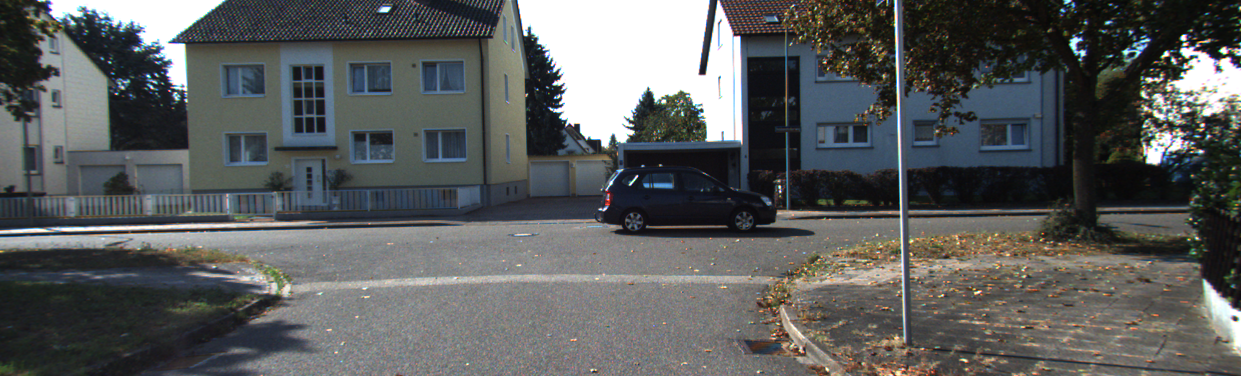
\includegraphics[width=\imwidth]{Data/KITTI/intersection}
				\end{subfigure}\hfill%
				\begin{subfigure}[b]{0.5\linewidth}
					\centering
					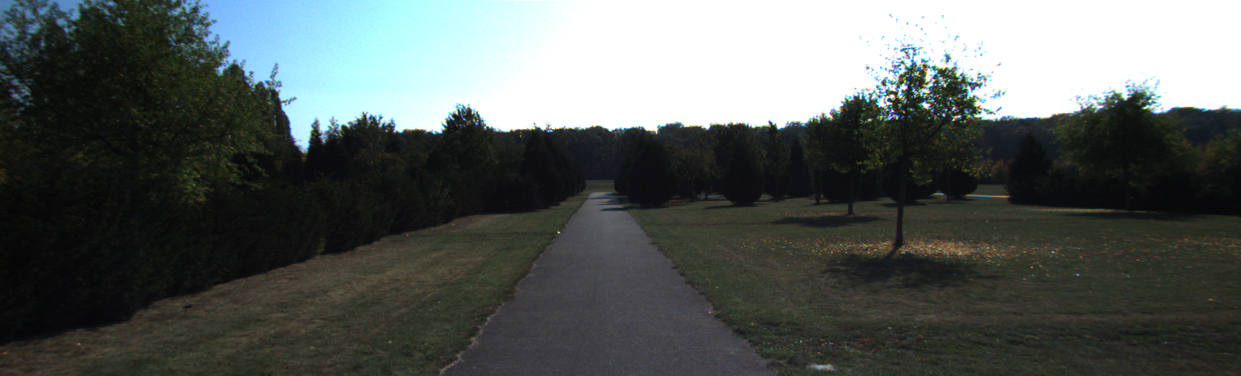
\includegraphics[width=\imwidth]{Data/KITTI/open-field}
				\end{subfigure}\hfill%
				\\
				\vspace{0.1cm}
				\begin{subfigure}[b]{0.5\linewidth}
					\centering
					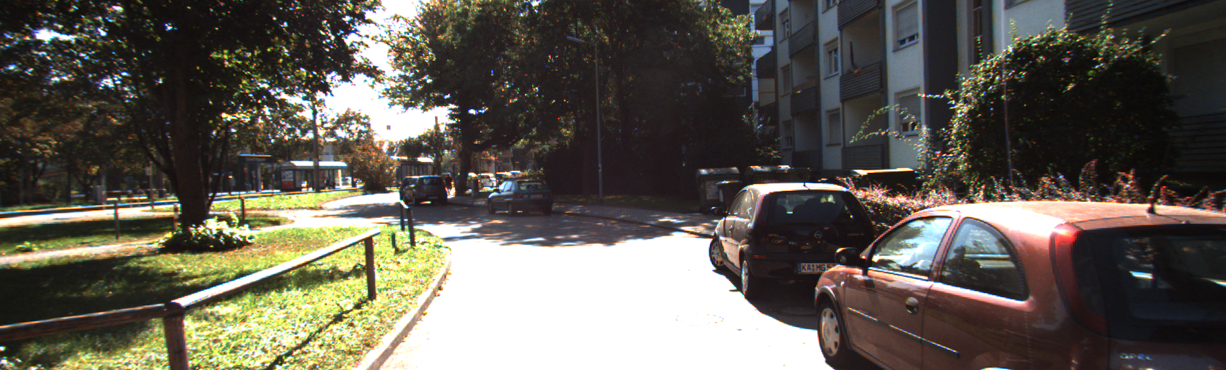
\includegraphics[width=\imwidth]{Data/KITTI/reflections-on-cars}
				\end{subfigure}\hfill%
				\begin{subfigure}[b]{0.5\linewidth}
					\centering
					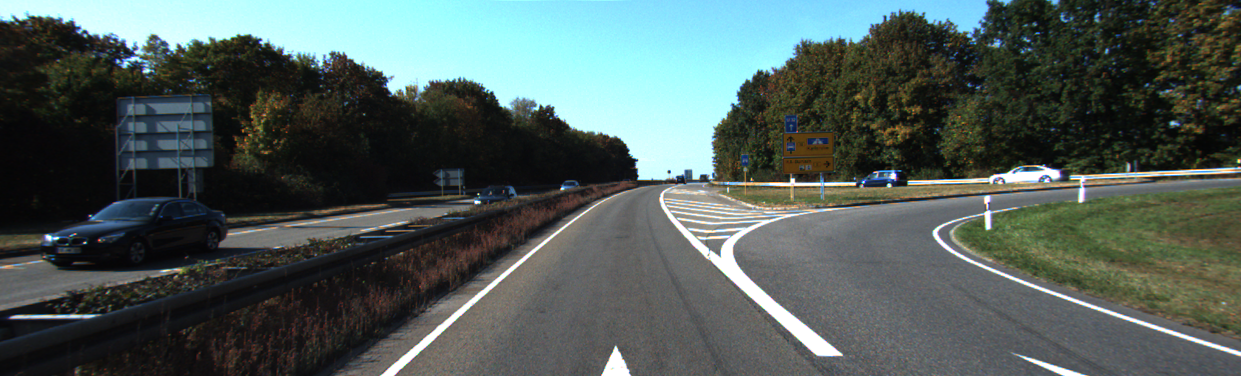
\includegraphics[width=\imwidth]{Data/KITTI/highway}
				\end{subfigure}\hfill%
				\caption[Example images from the KITTI dataset]
						{Example images from the KITTI dataset.
						 The pictures show wide open areas, narrow streets, reflections and moving cars.
						 The videos were captured with a camera mounted on top of a car.
						 \label{fig:example-images-from-KITTI}}
			\end{figure}
		
		\subsection{VIPER}
			The VIPER dataset from \cite{richter2017playing} contains a mix of car driving and walking sequences, but all data was generated synthetically from the video game Grand Theft Auto 5 (GTA V) for PC released in April 2015.
			With around 254k frames it is significantly larger that the KITTI dataset.
			There is a variety of ground truth data available, including camera pose, semantic class labels and 3D object bounding boxes.
			The camera poses have been directly extracted from the game engine and are therefore fully accurate, while other data such as the semantic labels were generated in a post-processing step.
			VIPER is subdivided into training, test, and validation sets with 134k, 70k, and 50k frames respectively.
			The splits contain diverse scenes at day and night across different scene types such as urban, suburban under various weather conditions.
			
		\subsection{GTA V}
			\todo{Maybe mention different types: standing, translation, etc.}
			The GTA V dataset, as presented in figure~\ref{fig:example-images-GTAV}, was created specifically for this thesis shortly before the VIPER dataset by \citeauthor{richter2017playing} was made public.
			Third party ``modding" tools%
			\footnote{\url{http://www.dev-c.com/gtav/}}
			had to be used to extract the camera pose information because the game developers do not intend users to modify the game files and only provide binaries for executing the software.
			The tool allows one to inject a user defined \CC\@ function to run code in a separate thread next to the game engine with access to variables such as the camera matrix, player- and world properties and more.
			The tool%
			\footnote{\url{https://github.com/awaelchli/GTA-V-Camera-Tracker}} 
			developed for this thesis streams the camera orientation and location to an output file with timestamps for each recorded pose.
			The video was recorded parallel to the pose with an external program called \emph{NVIDIA ShadowPlay}.
			Although both the recording of pose and video start synchronously, the rate at which the pose is queried is higher than the frame rate of the recorded video.
			Hence, the poses written to the output file were interpolated using the timestamps to match the 30 fps video recording.
			
			The dataset has a total of 470k frames of walking in first-person perspective.
			The sequences contain many factors of variation in form of weather changes (cloudy, sunny, night), dynamic motion of cars on the street or people on the sidewalk, different environments (urban, suburban, rural) and changes in speed (standing, walking, running).
			Although this dataset contains more video data compared to VIPER, it has only pose annotations.
			\begin{figure}
				\def\imheightv{2.2}
				\def\imheight{\imheightv cm}
				\def\imwidth{\fpeval{16/9*\imheightv}cm}
				\centering
				\begin{subfigure}[b]{0.33\linewidth}
					\centering
					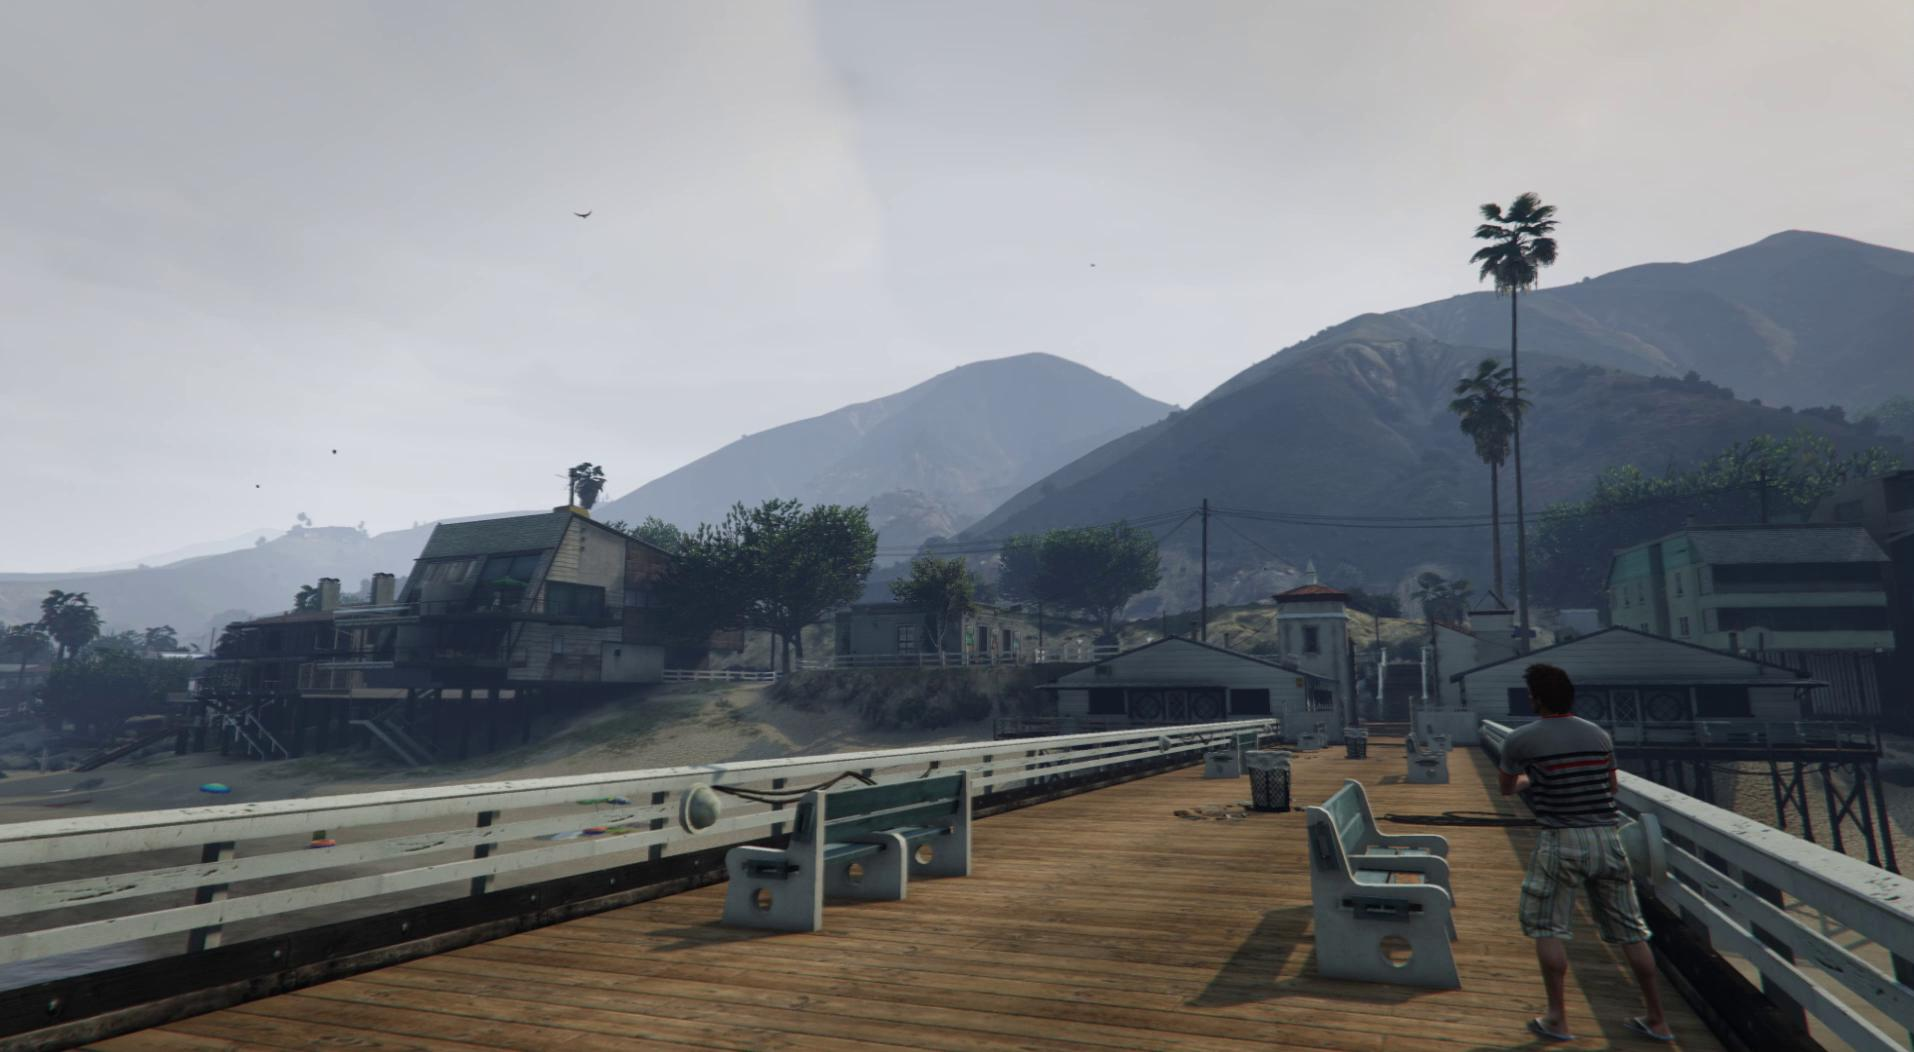
\includegraphics[height=\imheight, width=\imwidth]{Data/GTAV/pier-cloudy}
				\end{subfigure}\hfill%
				\begin{subfigure}[b]{0.33\linewidth}
					\centering
					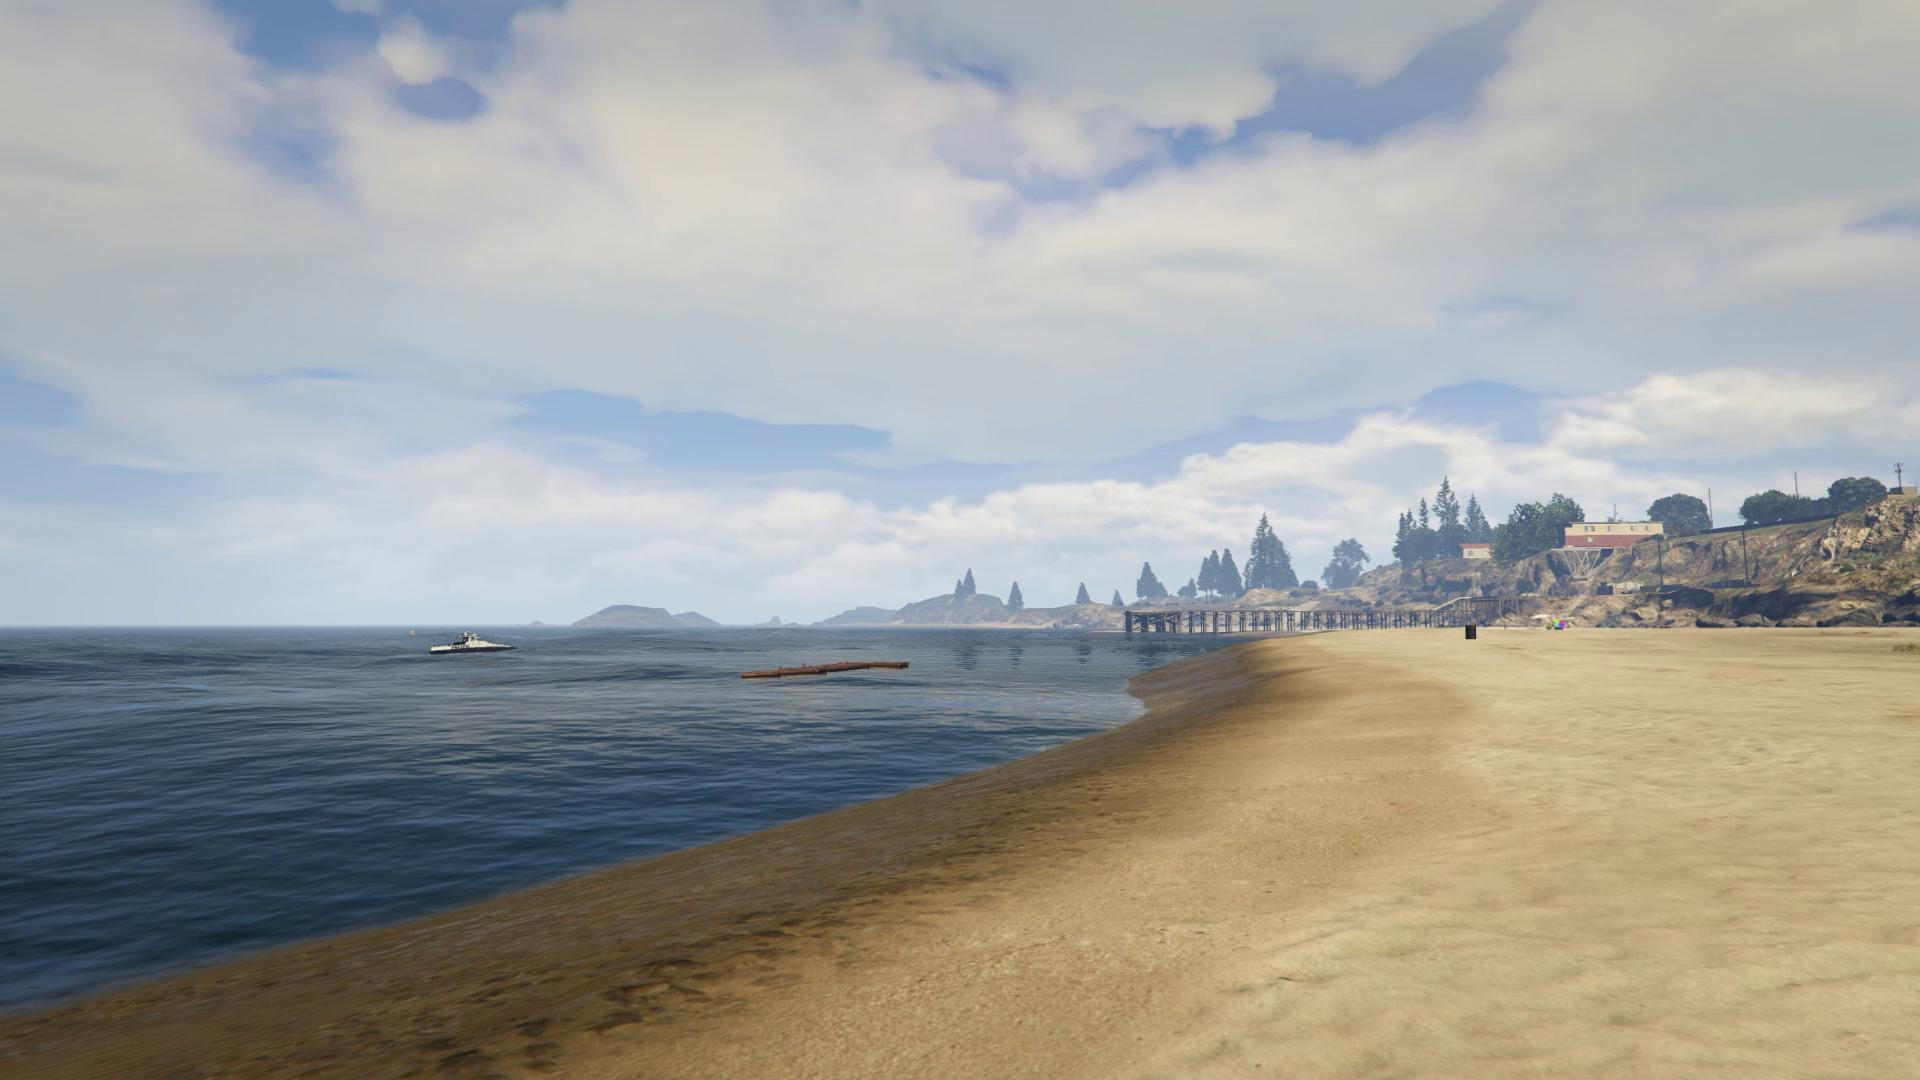
\includegraphics[height=\imheight, width=\imwidth]{Data/GTAV/beach}
				\end{subfigure}\hfill%
				\begin{subfigure}[b]{0.33\linewidth}
					\centering
					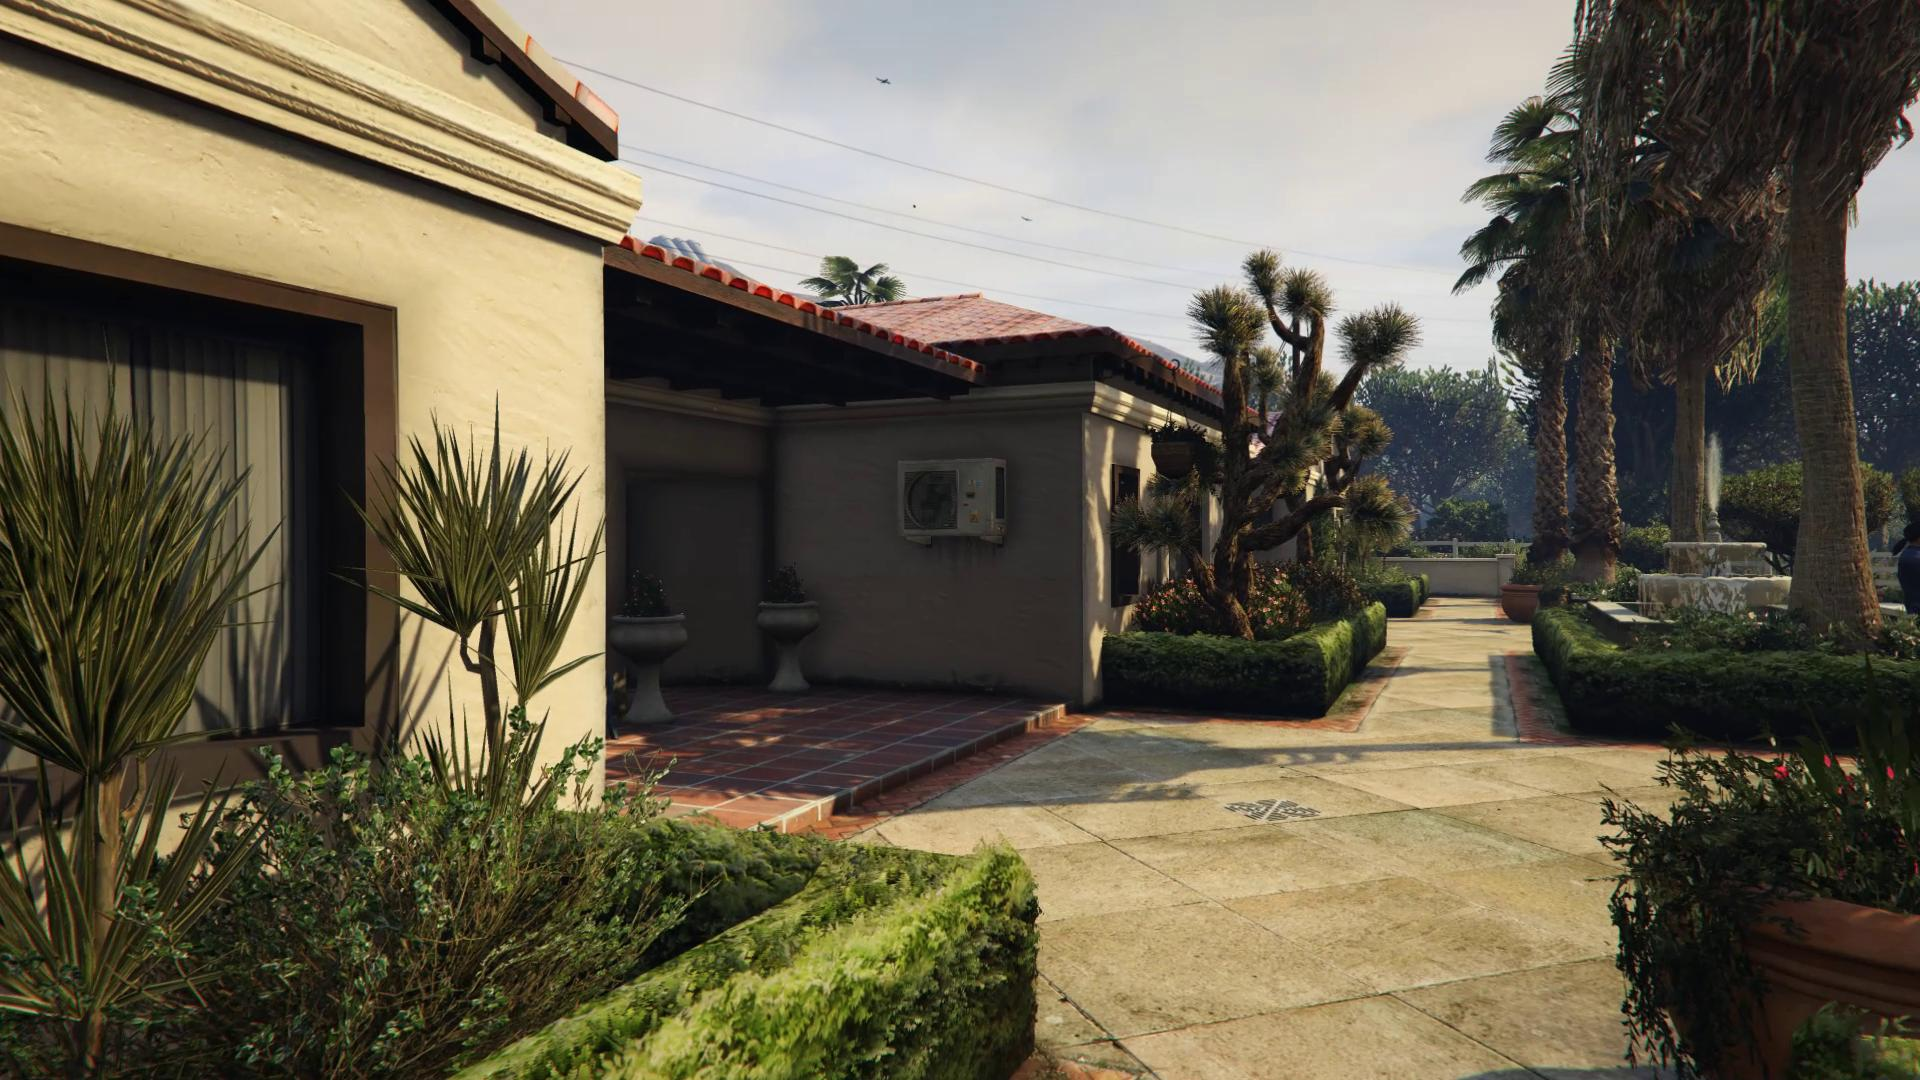
\includegraphics[height=\imheight, width=\imwidth]{Data/GTAV/garden-house}
				\end{subfigure}%
				\\
				\vspace{0.1cm}
				\begin{subfigure}[b]{0.33\linewidth}
					\centering
					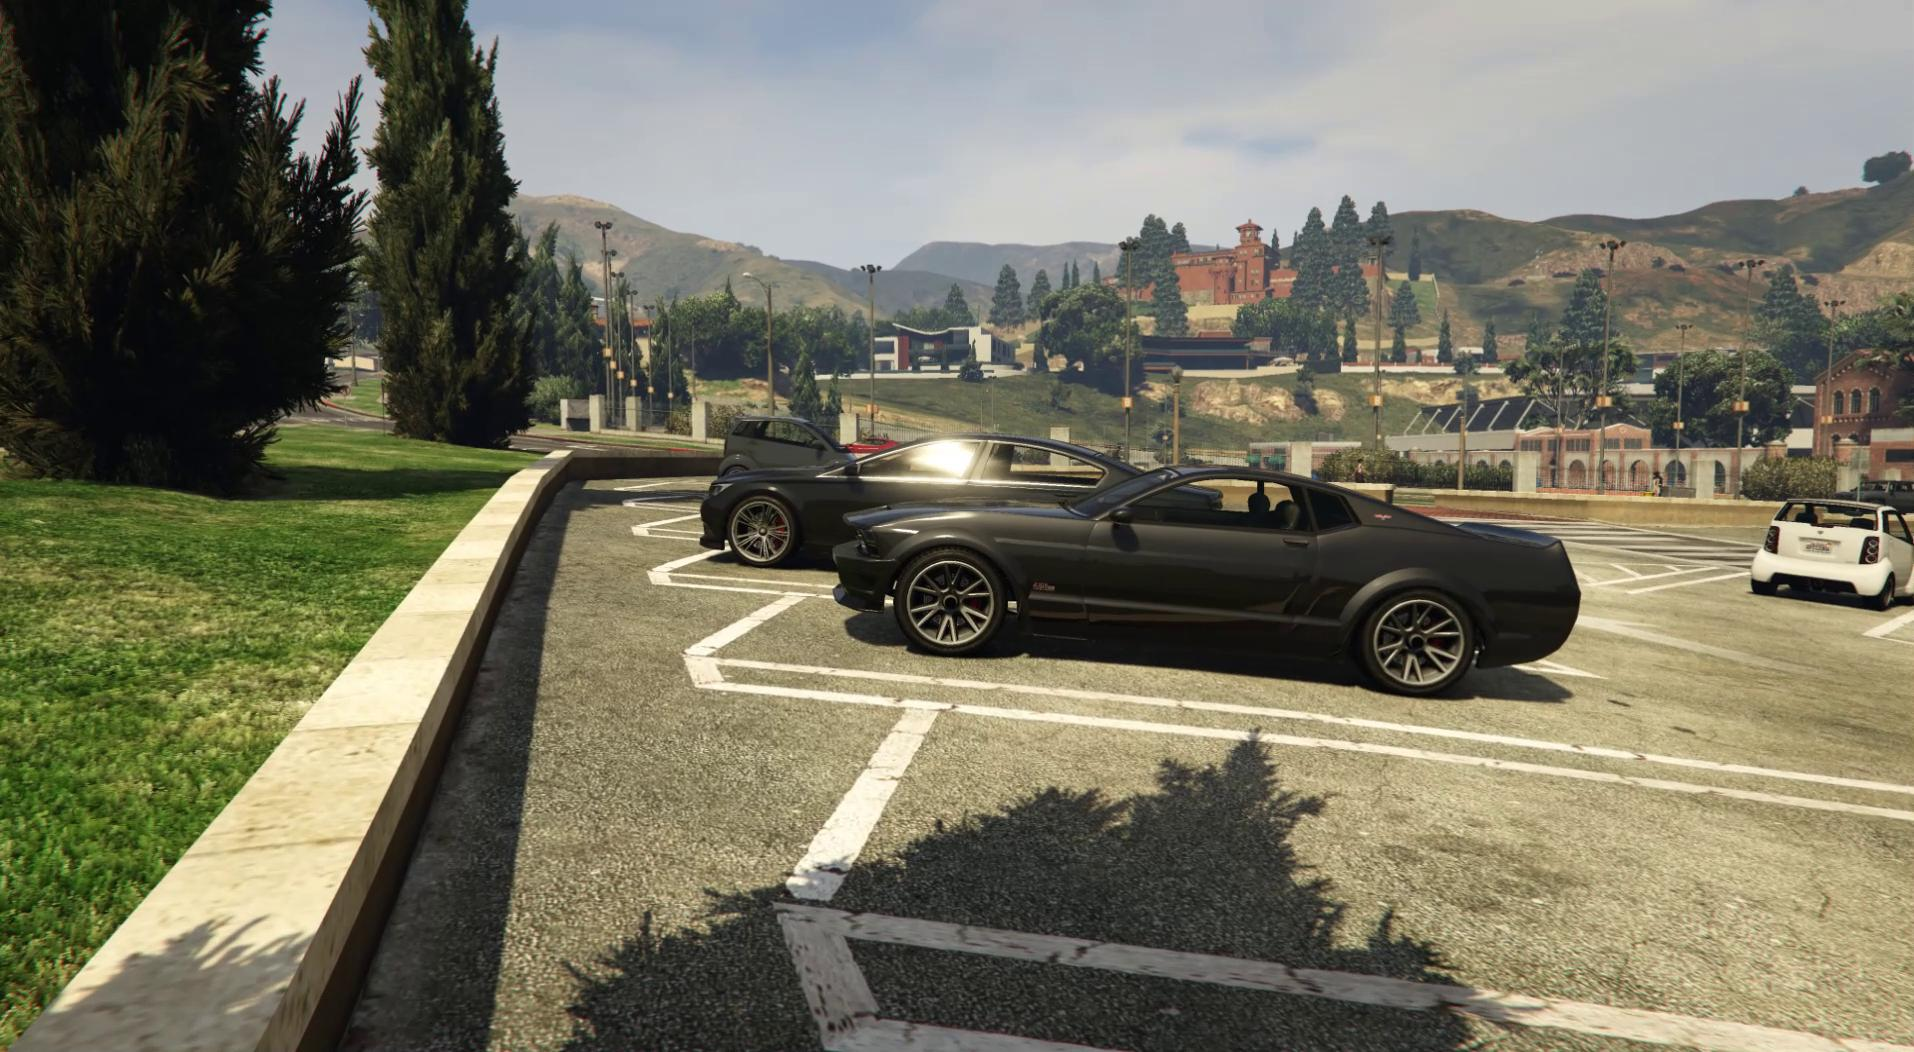
\includegraphics[height=\imheight, width=\imwidth]{Data/GTAV/parked-cars-reflections}
				\end{subfigure}\hfill%
				\begin{subfigure}[b]{0.33\linewidth}
					\centering
					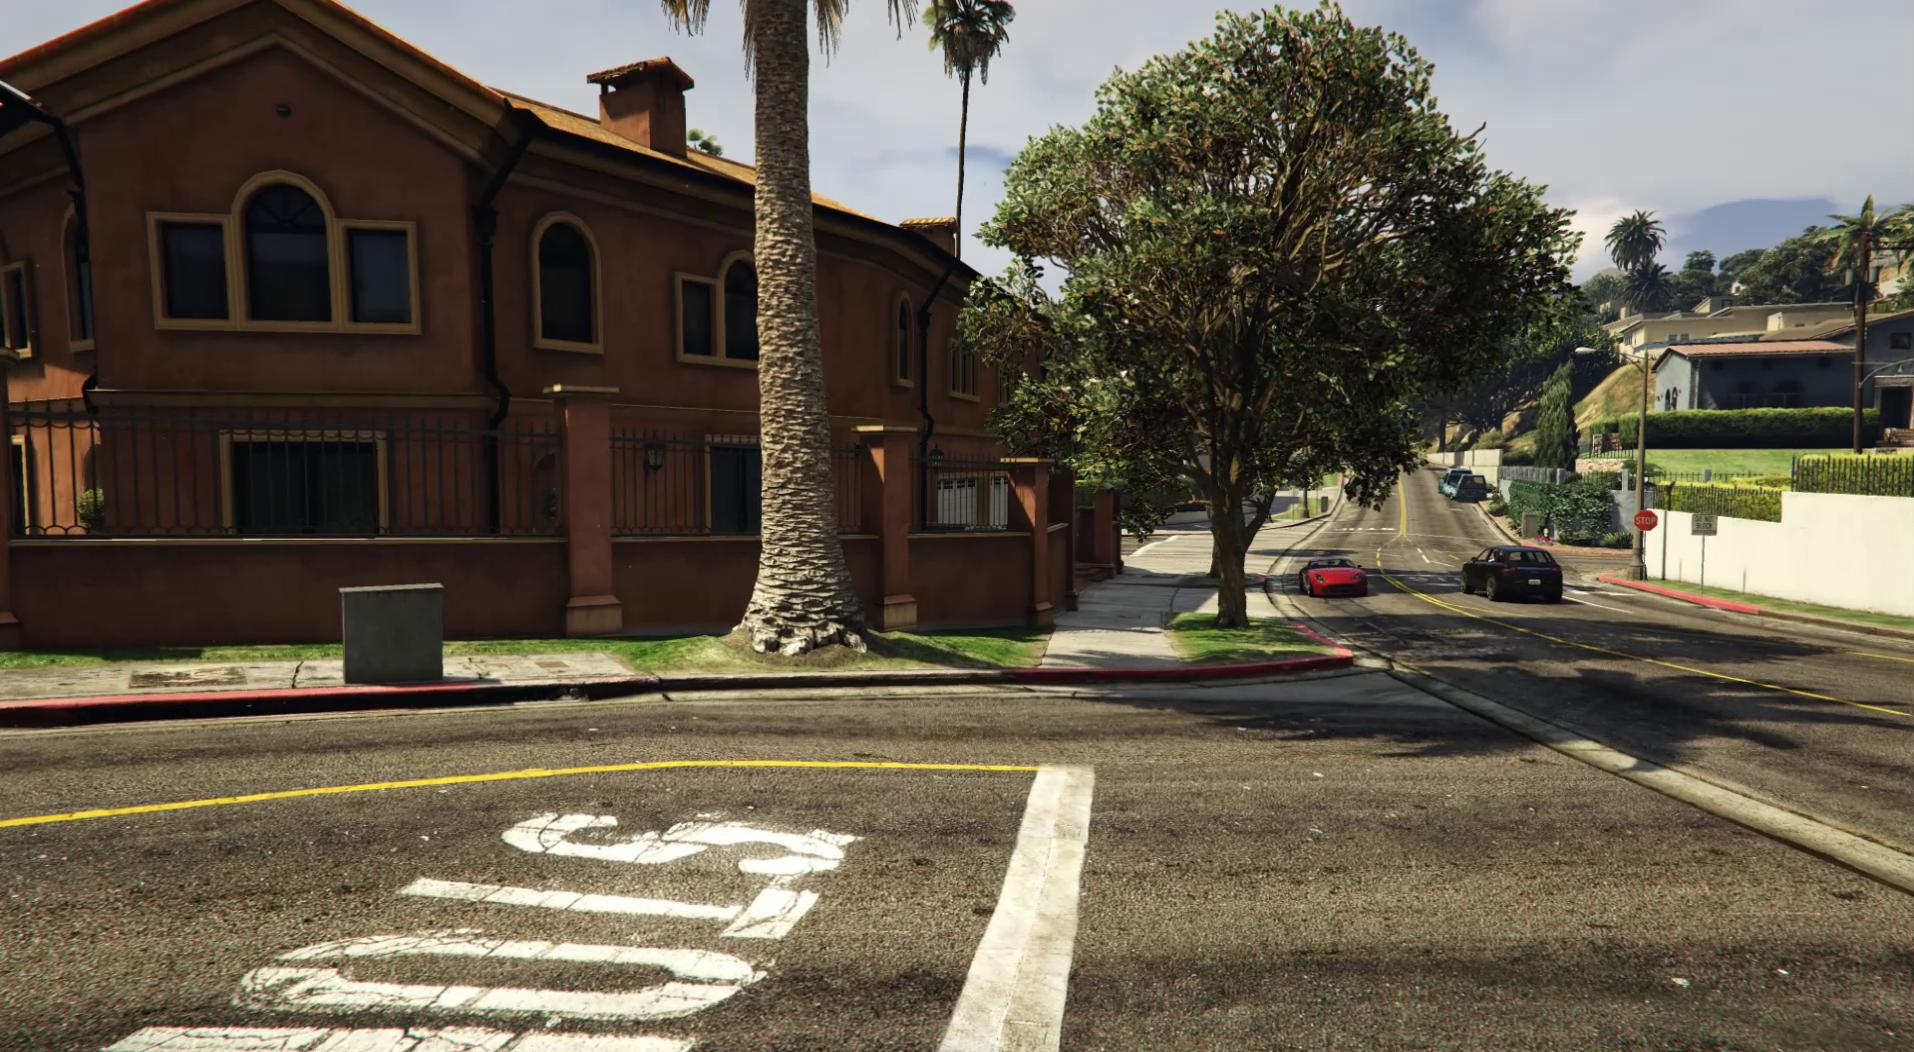
\includegraphics[height=\imheight, width=\imwidth]{Data/GTAV/suburban-sunny-streets}
				\end{subfigure}\hfill%
				\begin{subfigure}[b]{0.33\linewidth}
					\centering
					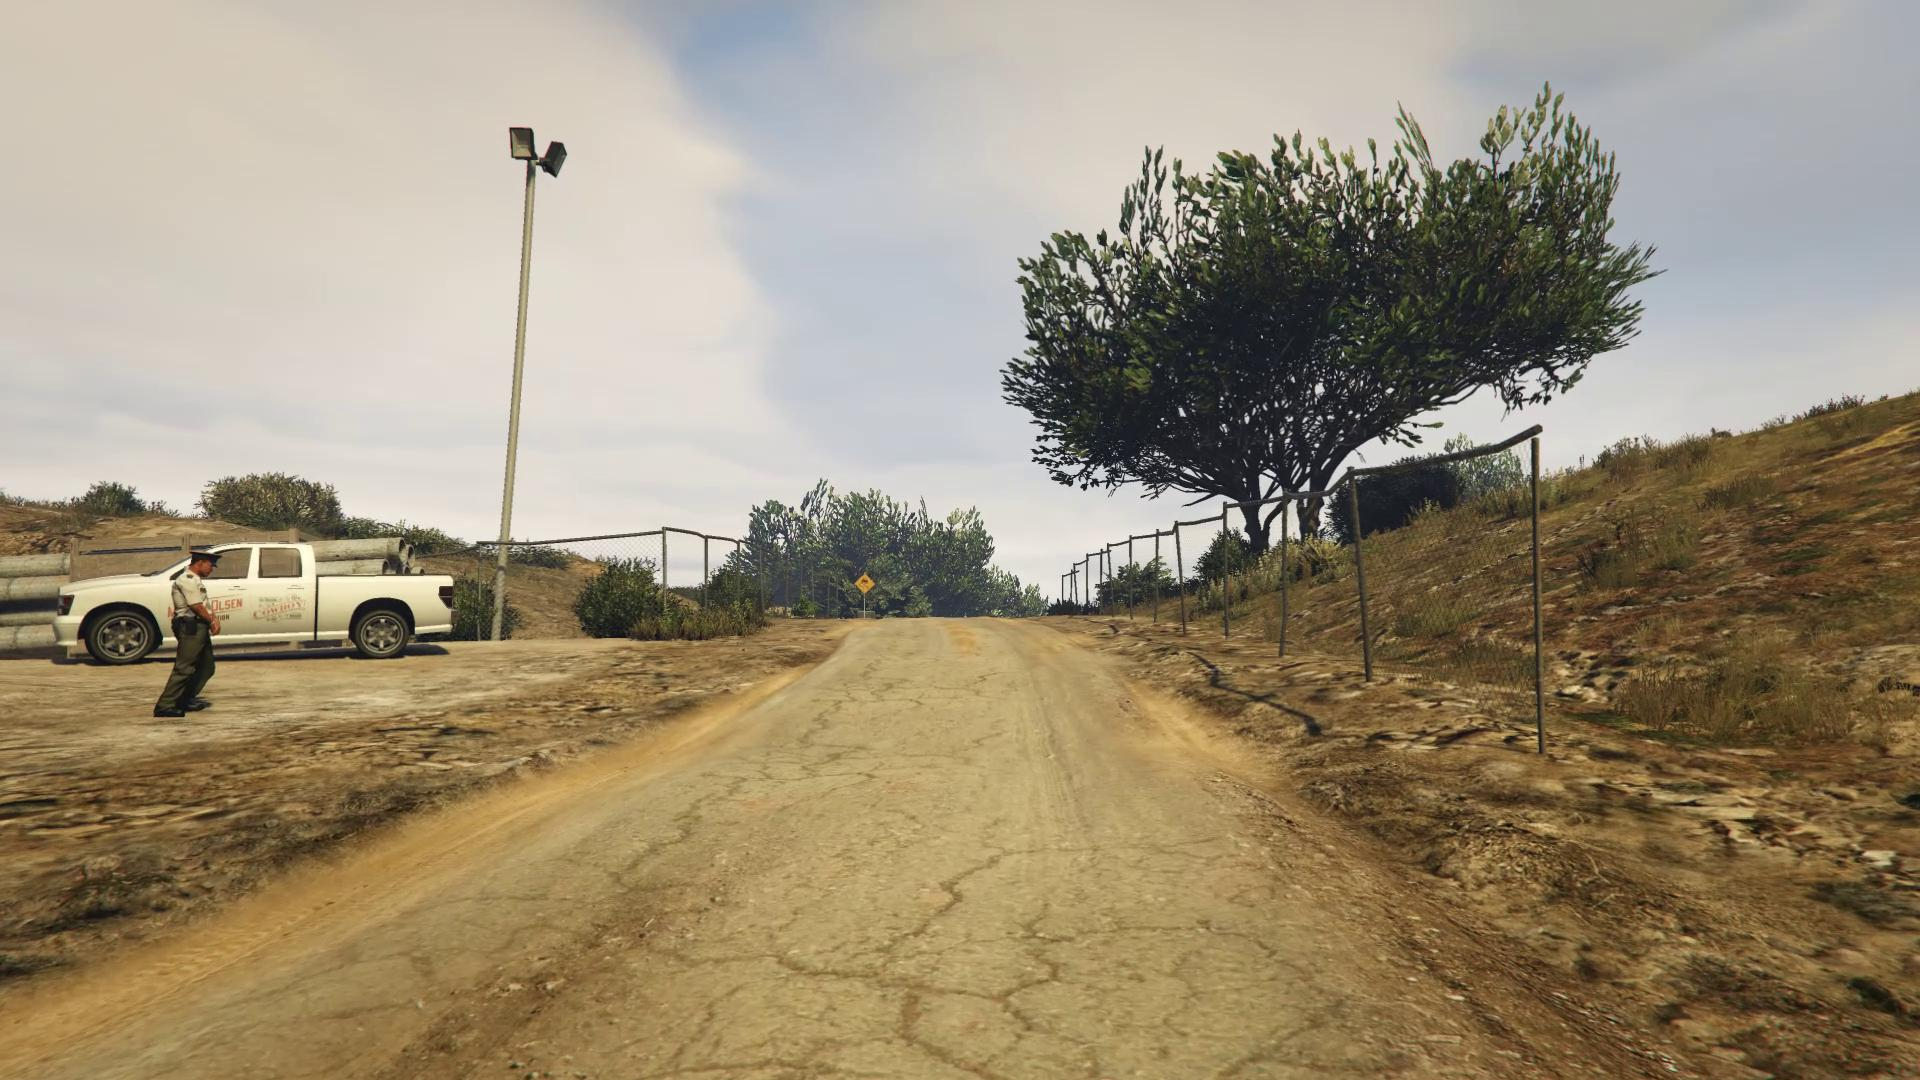
\includegraphics[height=\imheight, width=\imwidth]{Data/GTAV/desert-road}
				\end{subfigure}%
				\vspace{0.1cm}
				\begin{subfigure}[b]{0.33\linewidth}
					\centering
					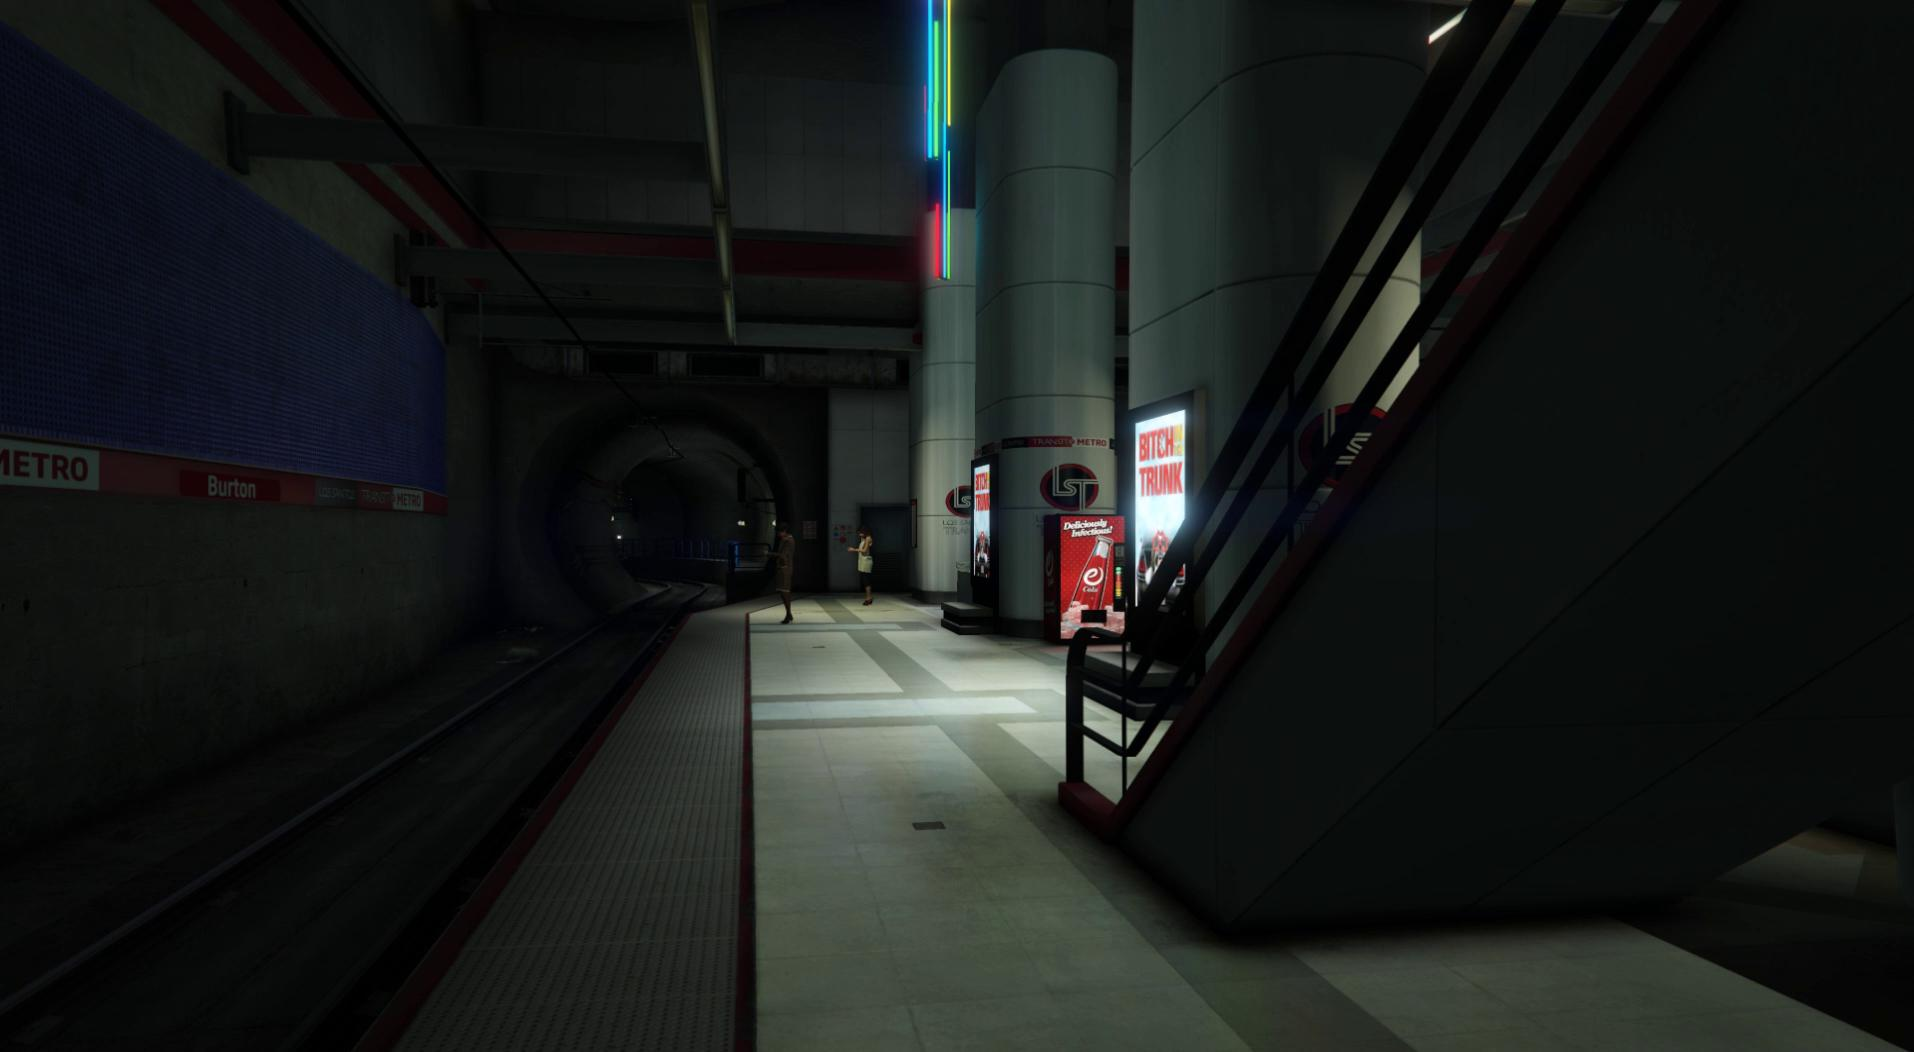
\includegraphics[height=\imheight, width=\imwidth]{Data/GTAV/metro}
				\end{subfigure}\hfill%
				\begin{subfigure}[b]{0.33\linewidth}
					\centering
					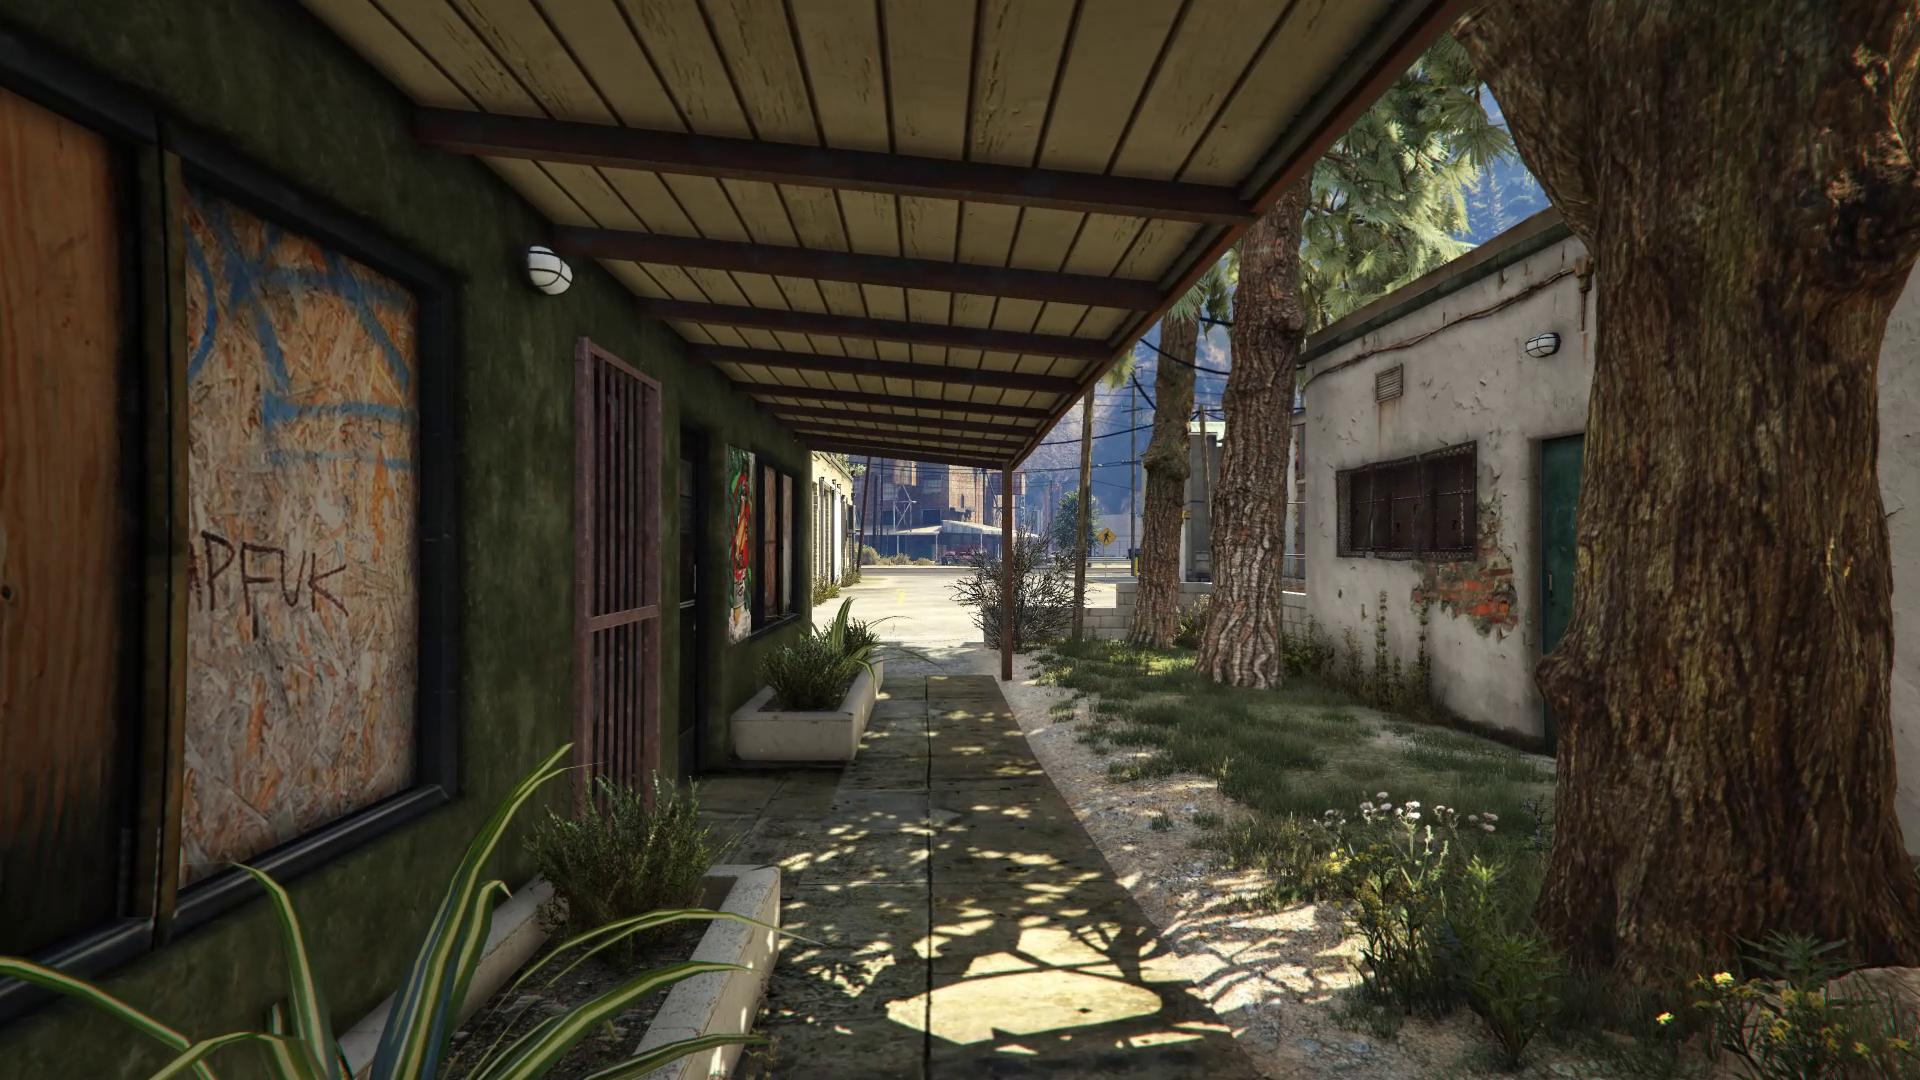
\includegraphics[height=\imheight, width=\imwidth]{Data/GTAV/close-shadows}
				\end{subfigure}\hfill%
				\begin{subfigure}[b]{0.33\linewidth}
					\centering
					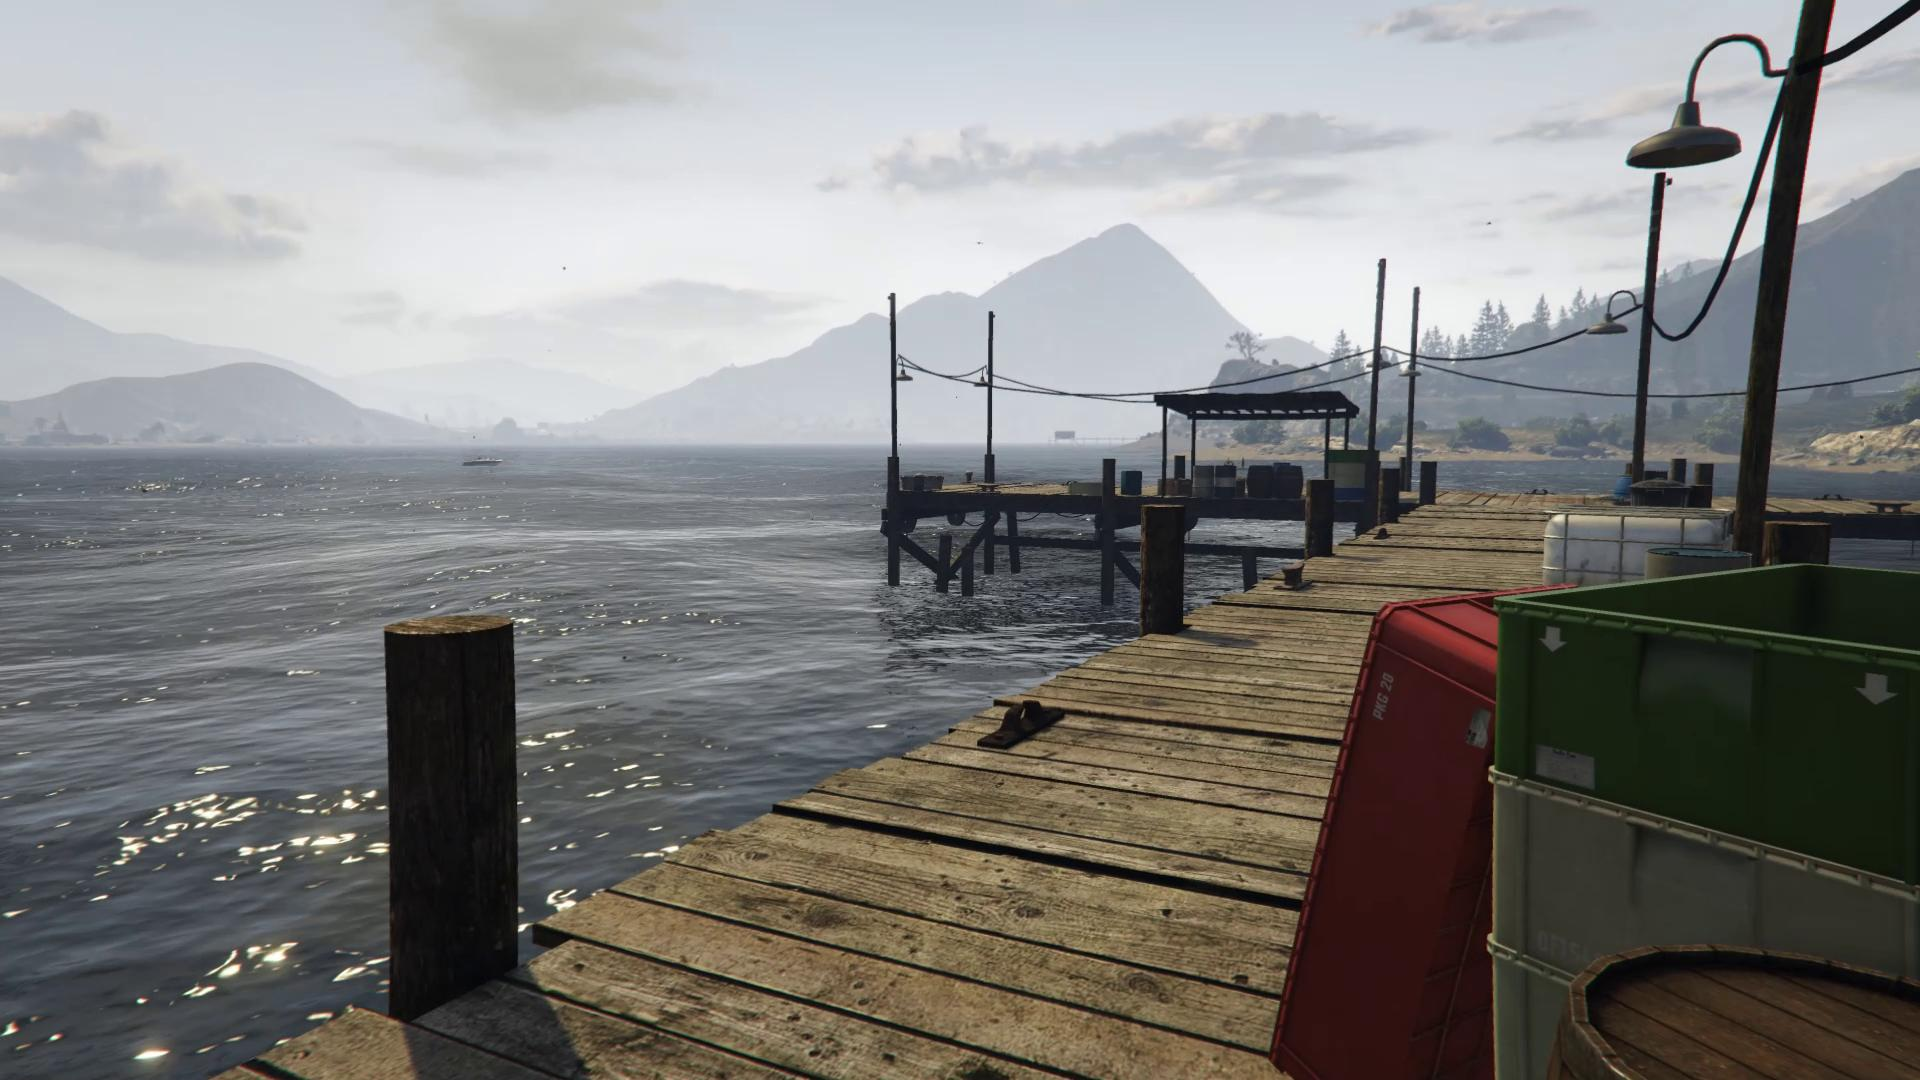
\includegraphics[height=\imheight, width=\imwidth]{Data/GTAV/pier-water-reflections}
				\end{subfigure}%
				\caption[Example images from the GTA V dataset]
						{Example images from different sequences in the GTA V dataset which was recorded for this thesis.
						 The images show wide open- as well as narrow places, reflections on cars and water, complex shadows from foliage and moving objects (people, cars).
						 \label{fig:example-images-GTAV}}
				%city-street-intersecton.jpg  
				%fountain-people.jpg  
				%desert-gas-station.jpg             
				%suburban-intersection.jpg
			\end{figure}
			
			
		\subsection{Preprocessing}\label{sec:preprocessing}
			Each dataset contains long sequences/videos of thousands of frames over several minutes of recording.
			Due to the high memory footprint, it is unfeasible to load a complete sequence and feed it to the network.
			Therefore the sequences are cut into subsequences of smaller sizes. 
			For most experiments here, the sequence size is 100 frames or less.
			Instead of creating a segmentation of the dataset, this method of extracting subsequences also allows to define an overlap between sequences.
			This is especially useful when the dataset is small, such as KITTI.
			
			Since resolution and aspect ratio of the images are different between the datasets, they are first proportionally resized to a height of 320 pixels and then the center region of $448 \times 320$ pixels is extracted.
			Fixing the input size across multiple datasets makes it possible to train the same network architecture for different data and make a more accurate comparison.
			Due to the cropping, the left and right boundaries of the image are removed.
			An alternative is to resize the images directly without regard to the aspect ratio.
			This leads to a loss in horizontal resolution which could impact the networks performance for horizontal motions, e.g., a rotation of the camera around the vertical axis.
			The alternative resizing method was not studied in this thesis, but the impact is expected to be minor.
			
			The ground truth poses also require preprocessing. 
			Each raw sequence has a corresponding text file that contains the $3 \times 4$ pose matrices for every frame.
			These poses are all relative to the coordinate system of the first frame in the sequence.
			In other words, the coordinate system of the first frame is the world coordinate system of all other frames in the sequence.
			Because the raw sequences are divided into subsequences, the ground truth poses need to be converted to poses that are relative to the first frame within each subsequence.
			The formulas in equation~\ref{eq:relative_rotation_conversion_general} from chapter~\ref{chp:foundations} are applied here.
			
			
	\section{Encoding the Pose}
	% Text from intro
	
	
	\section{The Model}
	% Figure with the entire pipeline
	% - Figure showing optical flow ??
	% Feature extraction
	%	- Optical flow
	%	- features relevant for motion
	%	- Flow alone is not enough
	% 	- Other high-level representation
	% Pose estimation
	%	- LSTM transforms feature to pose
	%	- Uses history from poses seen before to make current estimate more precise
	%	- 
	% Loss function and optimization
	% mse loss on euler + translation
	% experiments show that euler works best
	% 	
		The model is the key to solving the task.
		By adjusting the weights during the training phase, it learns a high-level representation of relevant information in the input that is needed to produce the desired output.
		In the case of visual odometry, we aim to learn a representation for motion.
		Specifically, the network has to be able to distinguish between dynamic motion in the scene and camera motion.
		\todo{Refer to challenges/ambiguities discussed in introduction...}
		The following two sections describe the two main parts of the model.
		The architecture of the full model is shown in figure~\ref{fig:main-architecture}.
		\begin{figure}[t]
			\centering
			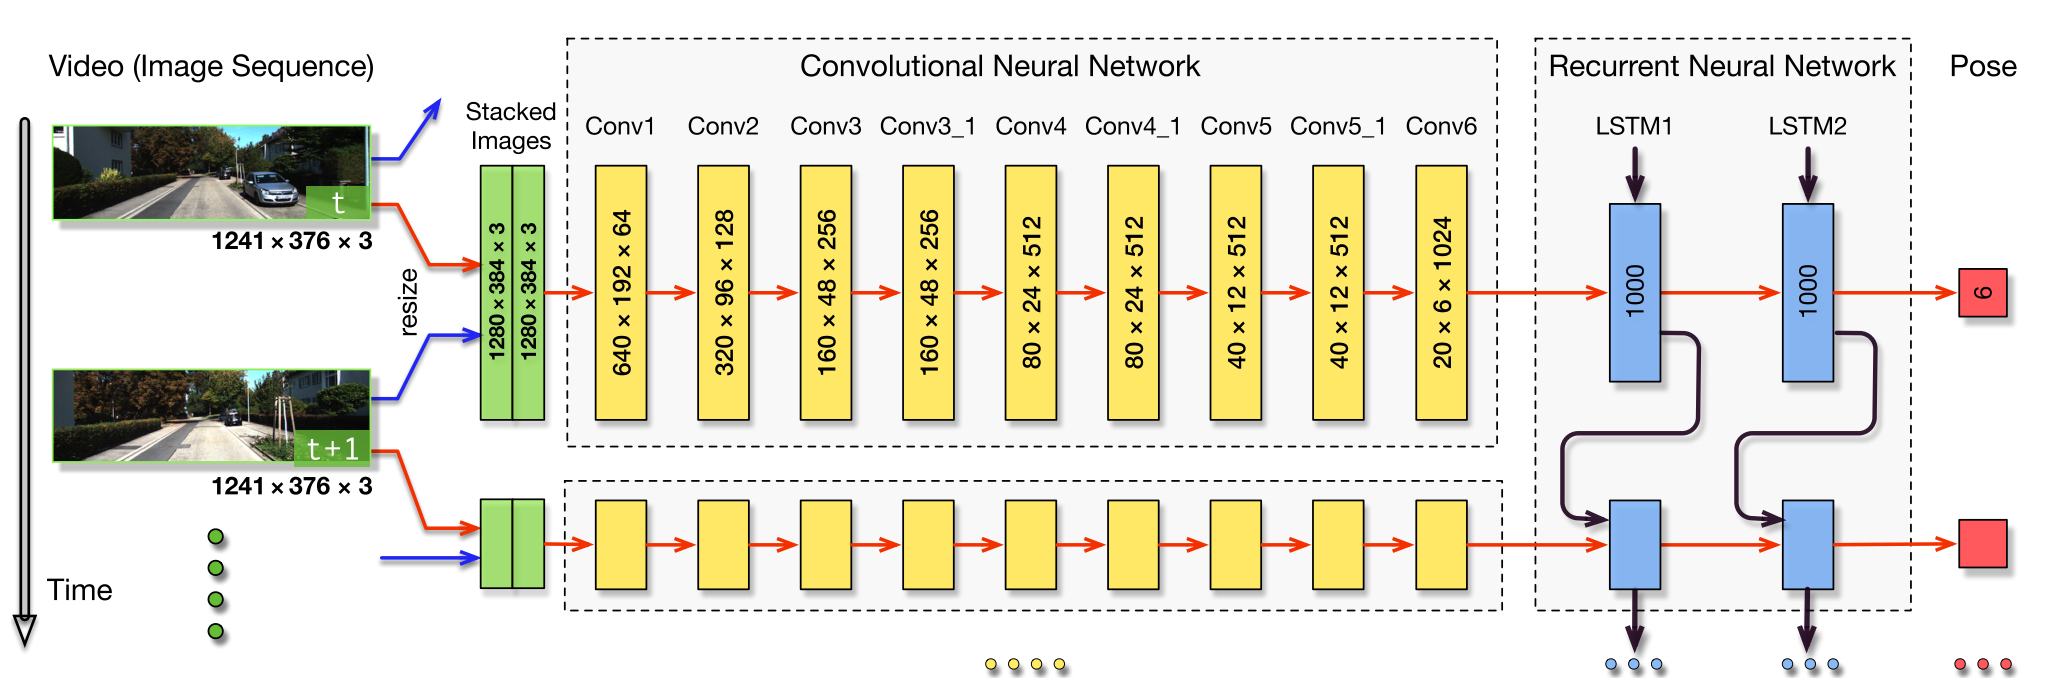
\includegraphics[width=\linewidth]{Model/DeepVO-arch}
			\caption[Main architecture for visual odometry]
					{Main architecture for visual odometry.
					 Green: Input of consecutive frames.
					 Yellow: Feature extraction.
					 Blue: Pose estimation with recurrent connections.
					 \todo{ref paper for figure, or redo figure}
					 \label{fig:main-architecture}}
		\end{figure}
		
		\subsection{Part 1: Feature Extraction}
			The purpose of the first part of the network is to extract information about motion from two consecutive frames at time $t$ and $t - 1$.
			One way to describe motion between two images is by \emph{optical flow}.
			It is defined as a vector-valued function $u(\vectr{x}) \in \R^2$ at each point $\vectr{x}$ in the image $I_{t}$ describing the translation of the point in the next frame such that
			\begin{equation}\label{eq:brightness_constancy_constraint}
				I_{t}(\vectr{x}) = I_{t + 1}(\vectr{x} + u(\vectr{x})).
			\end{equation}
			The property in equation~\ref{eq:brightness_constancy_constraint} is called the \emph{brightness constancy constraint}. 
			It means that a particular point can move in the image plane but it does not change its color.
			In general, this constraint does not hold for every point, e.g., because of occlusion introduced by motion.
			
			\cite{dosovitskiy2015flownet} describe a deep-learning approach for estimating optical flow.
			They propose and study two network architectures, \emph{FlowNetS} and \emph{FlowNetC}.
			The later is computing the inner product between patches of two input frames (correlation) followed by multiple layers of convolutions.
			FlowNetS on the other hand is the simple version that does not have the correlation layer. 
			Instead, it is only made of convolution layers and ReLUs.
			The first half of FlowNetS are strided convolutions that gradually increase the number of feature maps. 
			The second half, called refinement, consists of transposed convolution layers that, in reverse, increase the spatial dimension to form the high resolution optical flow maps.
			In addition, both FlowNet versions make use of skip-connections that allow the features from earlier layers to be added as input to layers in the second half by concatenating the tensors along the feature channel dimension. 
			
			In this thesis, the focus is on FlowNetS because it is the only publicly available implementation for PyTorch.\footnote{\citet*{flownetpytorch} has the source code available on GitHub.}
			FlowNetS is also the choice in the work of \citeauthor{wang2017deepvo}, which is the basis of the architecture described here.
			The FlowNetS implementation comes with pre-trained model weights.
			It is trained on a synthetic dataset of moving chairs rendered into images that serve as a static background.
			Although this data does not include camera motion, according to \citeauthor{wang2017deepvo} the model weights serve as a good initialization that leads to faster convergence. 
			
			Estimating camera motion solely based on optical flow is not very robust since scene motion is mixed into the optical flow which can significantly vary in magnitude.
			In order to have a more abstract representation, only the layers in the first half up to ``conv6.1'' are used for feature extraction.
			All layers in the second half of FlowNetS are dropped.
			The exact configuration of the remaining layers is shown in table~\ref{tbl:first_part_of_flownets}.
			\begin{table}[tb]
				\small
				\begin{center}
					\begin{tabular}{lcccc}
						\toprule
						Layer 		& Kernel size 		& Stride 		& Padding 		& Channels 		\\
						\midrule
						conv1 		& $7 \times 7$		& 2 			& 3 			& 64 			\\
						conv2 		& $5 \times 5$		& 2 			& 2 			& 128 			\\
						conv3 		& $5 \times 5$		& 2 			& 2 			& 256			\\
						conv3.1 	& $3 \times 3$		& 1 			& 1 			& 256 			\\
						conv4 		& $3 \times 3$		& 2 			& 1 			& 512 			\\
						conv4.1 	& $3 \times 3$		& 1 			& 1 			& 512 			\\
						conv5 		& $3 \times 3$		& 2 			& 1 			& 512 			\\
						conv5.1 	& $3 \times 3$		& 1 			& 1 			& 512 			\\
						conv6 		& $3 \times 3$		& 2 			& 1 			& 1024 			\\
						conv6.1 	& $3 \times 3$		& 1 			& 1 			& 1024 			\\
						\bottomrule
					\end{tabular}
				\end{center}
				\caption[Architecture of the feature extraction based on FlownetS]
						{Architecture of the feature extraction based on FlownetS. 
						 Each layer is a convolution followed by a rectified linear unit (ReLU).
						 \label{tbl:first_part_of_flownets}}
			\end{table}
			Note that the convolutions are applied with a stride and therefore the spatial size is reduced from one layer to the next.
			At the same time, the number of feature maps (channels) increases up to 1024 in the last layer.
			Say the input images have a width and height of $448 \times 320$ pixels, for example. 
			Then the output tensor contains 1024 feature maps of size $7 \times 5$.
			These activations are a coarse and abstract description of the motion seen in the input and do not directly imply the per-pixel optical flow.
			To emphasize again, we do not directly make use of optical flow since we are interested in separating camera motion from scene motion.
			This has to be done on a higher level of abstraction.
			The remaining task is now to take these coarse features and map them to the camera pose. 
			
		\subsection{Part 2: Pose Estimation}
		% How does LSTM use flow features 
		% Table with fc layer and dropout
			The key component of the second part is the LSTM that maps the motion features to a hidden state.
			Due to the recurrent connections, the hidden state does not only encode the pose at the current time step, but also a history of poses from previous time steps.
			To be clear, it is not obvious that the LSTM will actually learn a representation for the past and use that information to estimate the pose because nothing is explicitly forcing the network to do so.
			The question whether or not the recurrent connections make a significant contribution will be addressed in section~\ref{sec:odometry-experiments-and-results}.\todo{check ref}
			
			As opposed to convolution layers, the LSTM is defined in terms of matrix operations and hence the size of the input to the LSTM is not variable.
			This also implies that there is a limit on the size of the input images.
			As described in section~\ref{sec:preprocessing}, the images are rescaled to $448 \times 320$ pixels, which leads to a tensor of size $1024 \times 7 \times 5$ after feature extraction.
			This tensor is then reshaped to a vector with $1024 \cdot 7 \cdot 5 = 35840$ elements and fed to the LSTM as input.
			Although the LSTM itself applies multiple operations involving input, hidden state and gate outputs, it can be summarized as one single layer.
			Moreover, as shown in figure~\ref{fig:main-architecture} we adopt the architecture of~\citeauthor{wang2017deepvo} and stack two LSTM layers.
			Each of these recurrent layers has an associated hidden state of size $d = 1000$.
			
			The recurrent layers are followed by dropout and a fully connected layer that reduces the output size of the LSTM to a 6D vector for the pose.
			Table~\ref{tbl:lstm_and_fc_after_flownet} summarizes the input- and output dimensions of all layers in the second component of the network.
			\begin{table}[tb]
				\small
				\begin{center}
					\begin{tabular}{lcc}
						\toprule
						Layer 		& Input size 					& Output size			\\
						\midrule
						LSTM 1 		& $35840$						& $1000$  				\\
						LSTM 2 		& $1000$						& $1000$ 				\\
						drop		& $1000$						& $1000$				\\
						fc 			& $1000$						& $6$					\\
						\bottomrule
					\end{tabular}
				\end{center}
				\caption[Architecture of the recurrent part of the pose network]
						{Architecture of the recurrent part of the pose network.
						 It consists of a two-layer LSTM with hidden size 1000, a dropout- and fully-connected layer.
						 \todo{also include num parameters?}}
				\label{tbl:lstm_and_fc_after_flownet}
			\end{table}
		
		\subsection{Optimization}
			At each time step $t = 1, \dots, T$ the LSTM outputs a pose estimate 
			$\vectr{\hat{y}}_t = \left[ \, \vectr{\hat{p}}_t,  \vectr{\hat{\varphi}}_t \right]$.
			The quality of this estimate is determined by comparison against the ground truth pose 
			$\vectr{y}_t = \left[ \, \vectr{p}_t,  \vectr{\varphi}_t \right]$
			with the loss function
			\begin{equation}\label{eq:euler_pose_loss_function_t}
				\mathcal{L}_t(\vectr{y}_t, \vectr{\hat{y}}_t) = 
				%\sum_{t=1}^{T} 
					\lVert \vectr{p}_t - \vectr{\hat{p}}_t \rVert_2^2 + 
					\beta \lVert \vectr{\varphi}_t - \vectr{\hat{\varphi}}_t \rVert_2^2.
			\end{equation}
			As defined in equation~\ref{eq:loss_for_rnn}, the full loss of all estimates in the sequence is the sum of the losses in the sequence, i.e., 
			$\mathcal{L} = \sum_{t = 1}^{T} \mathcal{L}_t$.
			This loss function balances the squared error of position and Euler angles with a hyperparameter $\beta > 0$.
			The scale of positional change is usually higher than the angular changes for rotation, but in general, the scale depends on the ground truth provided in the dataset, e.g., the unit of measurements used or the speed of the camera motion.
			\cite{kendall2017geometric} find that $\beta$ requires significant tuning to get acceptable results.
			Moreover, as an alternative they propose a loss based on the reprojection error of the 3D points that naturally balances rotation and translation and therefore the need for manual balancing is eliminated.
			However, this thesis does not explore a geometric loss function of this type.
			The balance value in equation~\ref{eq:euler_pose_loss_function_t} is manually chosen and set to $\beta = 10$ by default for training.
			For evaluation on the test set in all experiments that follow, we use $\beta = 1$.
			Furthermore, the two terms 
			$\lVert \vectr{p}_t - \vectr{\hat{p}}_t \rVert_2^2$ and 
			$\lVert \vectr{\varphi}_t - \vectr{\hat{\varphi}}_t \rVert_2^2$
			in equation~\ref{eq:euler_pose_loss_function_t} are referred to as the translation- and rotation errors respectively.
			
			\todo{Mention choice of beta in experiments section}
			
			For training, the Adam optimizer is used with default settings and initial learning rates $\lambda_1 = 10^{-4}$ and $\lambda_2 = 10^{-3}$ for each part of the network.
			$\lambda_1$ is the learning rate for the part that is initialized with weights from a pre-trained FlowNetS.
			It is chosen to be smaller than $\lambda_2$ because the transferred weights are expected to be already close to optimal values and can be fine-tuned with a smaller learning rate.
			\todo{Mention (maybe in discussion) the difference of this training technique to deepvo paper.}
			
			
			
	\section{Implementation}
		PyTorch is a deep learning framework for Python that comes with a rich tensor library.
		It differs from other libraries (TensorFlow, Caffe, Theano and more) in the sense that it builds the computational graph dynamically at runtime.
		This flexibility allows for controlling the computational flow while training or testing the network.


	\newpage{\pagestyle{empty} \cleardoublepage}
	
	
	\begin{appendix}
		\chapter{Appendix}

		\newpage{\pagestyle{empty} \cleardoublepage}
	\end{appendix}
	
	\addcontentsline{toc}{chapter}{\numberline{}List of Tables}
	\listoftables
	
	\addcontentsline{toc}{chapter}{\numberline{}List of Figures}
	\listoffigures
	
	\addcontentsline{toc}{chapter}{\numberline{}Bibliography}
	\bibliographystyle{alphadin}
	%\bibliographystyle{plainnat}
	\nocite{*}
	\bibliography{thesis}
	\todo{check spelling, capitalization and dates of references}
	
	% This is required since 2012!!
	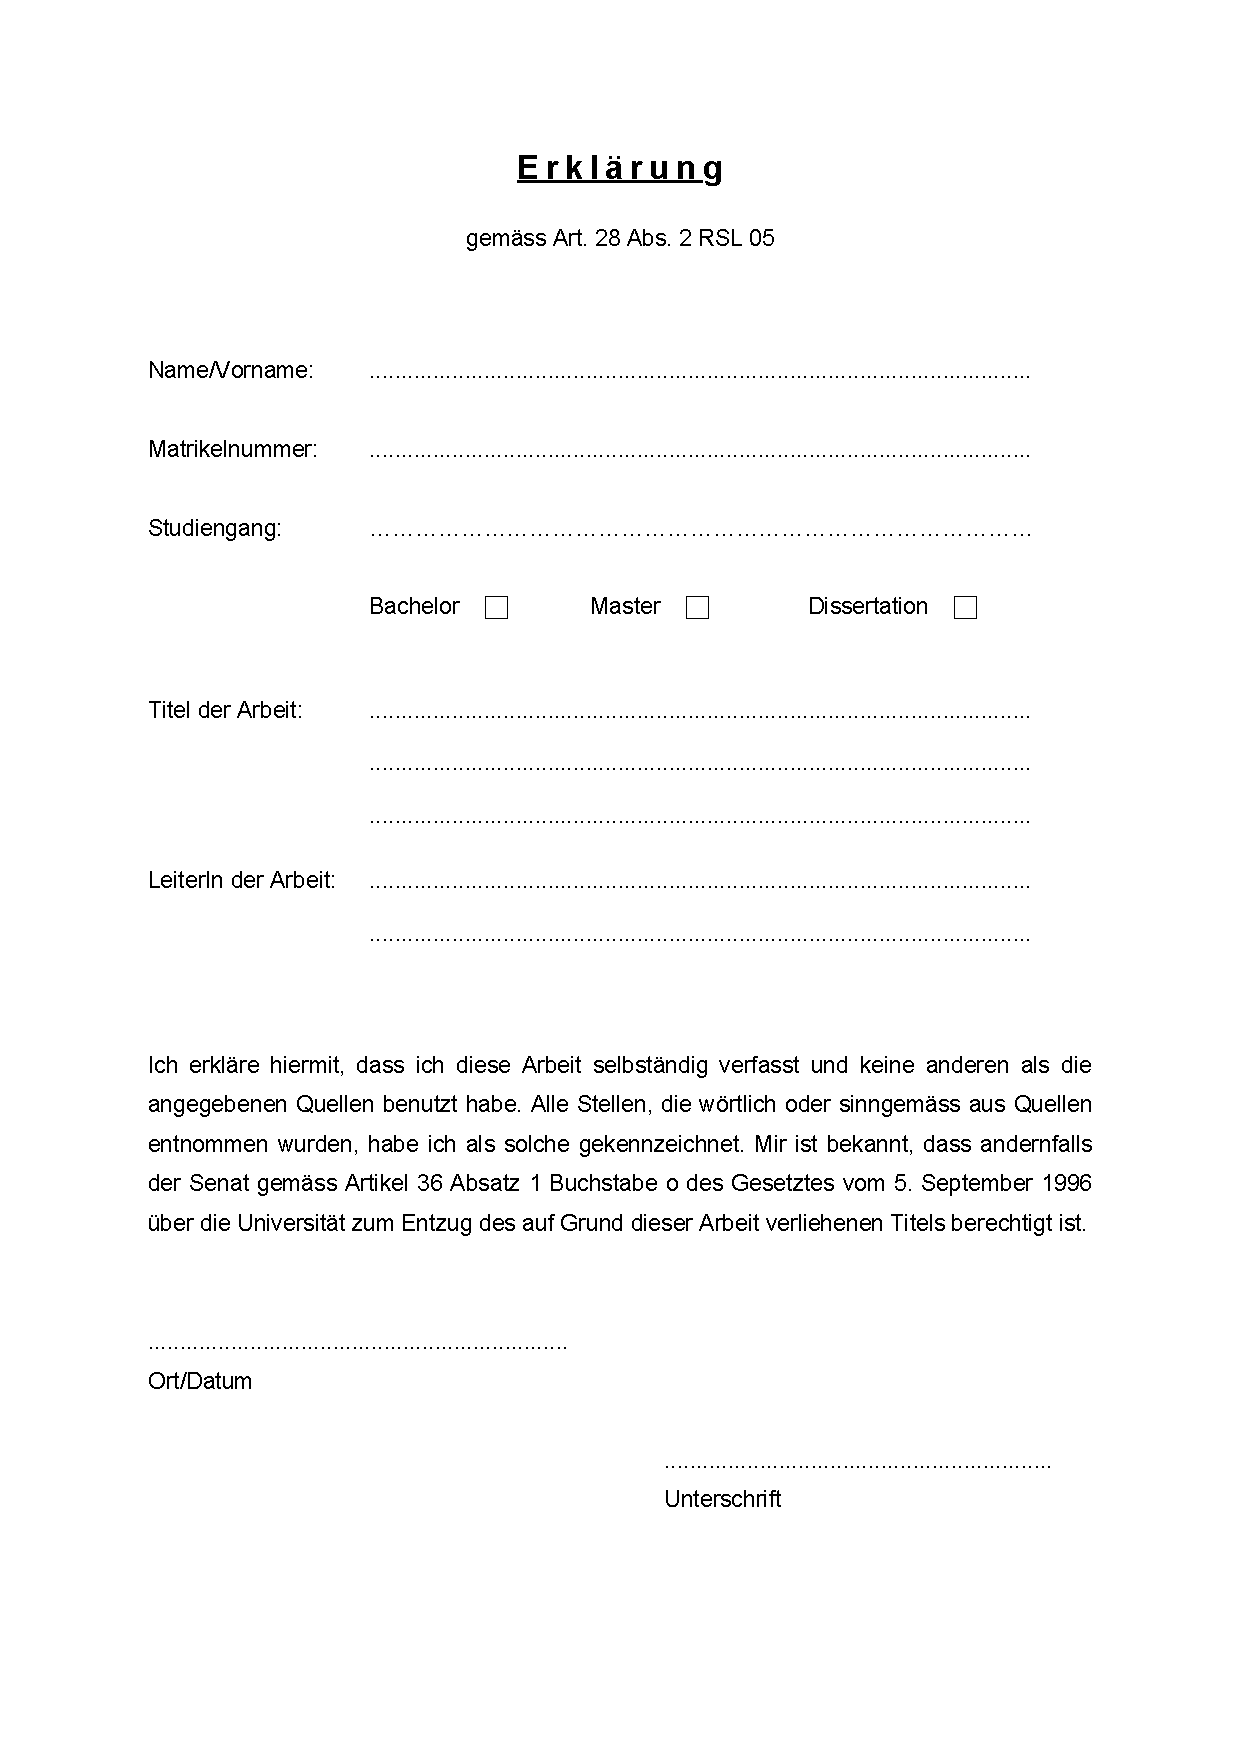
\includepdf{Erklaerung.pdf}

\end{document}
